% Copyright 2007, 2008, 2009 Elsevier Ltd
%
% This file is part of the 'Elsarticle Bundle'.
% ---------------------------------------------
%
% It may be distributed under the conditions of the LaTeX Project Public
% License, either version 1.2 of this license or (at your option) any
% later version.  The latest version of this license is in
%    http://www.latex-project.org/lppl.txt
% and version 1.2 or later is part of all distributions of LaTeX
% version 1999/12/01 or later c.
%
% The list of all files belonging to the 'Elsarticle Bundle' is
% given in the file `manifest.txt'.
%

% Template article for Elsevier's document class `elsarticle'
% with harvard style bibliographic references
% SP 2008/03/01
%
%
%
% $Id: elsarticle-template-harv.tex 4 2009-10-24 08:22:58Z rishi $
%
%
\documentclass[preprint,authoryear,12pt]{elsarticle}

% Use the option review to obtain double line spacing
%\documentclass[authoryear,preprint,review,12pt]{elsarticle}

% Use the options 1p,twocolumn; 3p; 3p,twocolumn; 5p; or 5p,twocolumn
% for a journal layout:
%\documentclass[final,authoryear,1p,times]{elsarticle}
%\documentclass[final,authoryear,1p,times,twocolumn]{elsarticle}
%\documentclass[final,authoryear,3p,times]{elsarticle}
%\documentclass[final,authoryear,3p,times,twocolumn]{elsarticle}
%\documentclass[final,authoryear,5p,times]{elsarticle}
%\documentclass[final,authoryear,5p,times,twocolumn]{elsarticle}

%% if you use PostScript figures in your article
%% use the graphics package for simple commands
%% \usepackage{graphics}
%\usepackage{cases}
%% or use the graphicx package for more complicated commands
\usepackage{graphicx}
%% or use the epsfig package if you prefer to use the old commands
\usepackage{epsfig}

\usepackage{comment}

\usepackage{epstopdf}
\usepackage{pdflscape}
\usepackage{bm}
\usepackage{hyperref,url}
\hypersetup{colorlinks=true, urlcolor=blue, linkcolor=blue, citecolor=red}

%% The amssymb package provides various useful mathematical symbols
\usepackage{amssymb,amsmath,array}
%The amsthm package provides extended theorem environments
\usepackage{amsthm}
\usepackage{graphicx}
\usepackage{subfigure}  
%% The lineno packages adds line numbers. Start line numbering with
%% \begin{linenumbers}, end it with \end{linenumbers}. Or switch it on
%% for the whole article with \linenumbers after \end{frontmatter}.
%% \usepackage{lineno}

\usepackage{lscape}

%% natbib.sty is loaded by default. However, natbib options can be
%% provided with \biboptions{...} command. Following options are
%% valid:

%%   round  -  round parentheses are used (default)
%%   square -  square brackets are used   [option]
%%   curly  -  curly braces are used      {option}
%%   angle  -  angle brackets are used    <option>
%%   semicolon  -  multiple citations separated by semi-colon (default)
%%   colon  - same as semicolon, an earlier confusion
%%   comma  -  separated by comma
%%   authoryear - selects author-year citations (default)
%%   numbers-  selects numerical citations
%%   super  -  numerical citations as superscripts
%%   sort   -  sorts multiple citations according to order in ref. list
%%   sort&compress   -  like sort, but also compresses numerical citations
%%   compress - compresses without sorting
%%   longnamesfirst  -  makes first citation full author list
%%
%% \biboptions{longnamesfirst,comma}

% \biboptions{}

\newcommand{\JGnote}[1]{\fbox{\parbox{\textwidth}{ \color{red} JG Note $\Rightarrow$ #1}}}
\newcommand{\KCnote}[1]{\fbox{\parbox{\textwidth}{ \color{black} KC Note $\Rightarrow$ #1}}}
\newcommand{\red}{\textcolor{red}}
\newcommand{\blue}{\textcolor{blue}}
\newcommand{\green}{\textcolor{green}}
\journal{Advances in Water Resources}
\newcommand{\frc}{\displaystyle\frac}
\newcommand{\PN}[2][error]{P$_{#1}$DG-P$_{#2}$}
\newcommand{\PNDG}[2][error]{P$_{#1}$DG-P$_{#2}$DG}

\begin{document}

\begin{frontmatter}

%% Title, authors and addresses

%% use the tnoteref command within \title for footnotes;
%% use the tnotetext command for the associated footnote;
%% use the fnref command within \author or \address for footnotes;
%% use the fntext command for the associated footnote;
%% use the corref command within \author for corresponding author footnotes;
%% use the cortext command for the associated footnote;
%% use the ead command for the email address,
%% and the form \ead[url] for the home page:
%%
%% \title{Title\tnoteref{label1}}
%% \tnotetext[label1]{}
%% \author{Name\corref{cor1}\fnref{label2}}
%% \ead{email address}
%% \ead[url]{home page}
%% \fntext[label2]{}
%% \cortext[cor1]{}
%% \address{Address\fnref{label3}}
%% \fntext[label3]{}

\title{ \blue{Numerical investigation of viscous flow instabilities through heterogeneous porous media using adaptive and unstructured meshes under different mobility scenarios - change the title to something close to the main topic of the manuscript ... something with viscous flow instability or viscous fingering)}}

%% use optional labels to link authors explicitly to addresses:
\author[UoA]{K. Christou} \author[UoA,UFRGS]{W.C. Rad\"unz}  \author[UoA]{B. Lashore} \author[UESC]{F.B.S. de Oliveira}
\author[UoA]{J.L.M.A. Gomes\corref{cor1}}\ead{jefferson.gomes@abdn.ac.uk}

\cortext[cor1]{Corresponding author.}
\address[UoA]{Environmental and Industrial Fluid Mechanics Group, School of Engineering, University of Aberdeen, UK}
\address[UFRGS]{Engineering School, Federal University of Rio Grande do Sul, Brazil}
\address[UESC]{Department of Exact and Technological Sciences, State University of Santa Cruz, Bahia, Brazil}

\begin{abstract} 
\KCnote{ \blue{......numerical modelling of multiphase flow in porous media has a wide range of applications in science and engineering. Viscous fingering, a fluid instability can be a major concern regarding enhanced oil-recovery methods (EOR). Continuity equation and the Darcy's law govern the processes, while pressure, velocity, saturation and permeability are quantities that define the behaviour of the flow. A novel control finite element method (CVFEM) is used to discretize the governing equations that will solve the multi-fluid porous media flow model. The current model is the basis of a general purpose flow simulator that is equipped with anisotropic mesh adaptivity techniques to increase the computational accuracy of numerical methods used in geophysical fluid mechanics and tackle the difficulties that commercial resevoir simulators may rise when using low order finite volume/differences methods based on structured grids. The governing multiphase porous media flow equations are solved using an adaptive and unstructured mesh. The model is based upon two key numerical characteristics: (a) the family of $P_{n}DG-P_{n+1}$ finite element pairs and (b) a consistent overlapping control volume finite element method (CVFEM) formulation.
%Moreover, the mesh adaptivity algorithm employs multi-constraints on element size in different regions of the porous medium to resolve multi-scale transport phenomena. The scheme captures the key characteristics of the flow while its applicable to heterogeneous porous media and geological formations. We conclude that understanding the multiphase flow properties will allow us to efficiently facilitate more efficient oil \& gas recovery, efficient contaminant removal and better planning of carbon capture and storage (CCS) projects.
In this paper the use of dynamic mesh adaptivity to capture the viscous fingering in reservoir flows is introduced, as one of the methods that will allow the user to focus the effort where is needed, minimizing both the CPU time and the numerical diffusion. Both the evolution of visualisation techniques through the extensive use of parallel computing as well as the advances in modelling and simulation of porous media flows may help to address the importance of this phenomenon which can be found in petroleum, chemical and environmental operations.
The aim of this paper is to extend and further apply the formulation (embedded in the Fluidity software framework) to multiphase flows in heterogeneous porous media combined with either uniform or random generated permeability distribution...}}

%\JGnote{ Abstracts for journal papers have very `squared-structure': (a) Motivation (why would anyone bother to read the paper? Why is it (the paper and/or the subject) relevant? This needs to be covered in 1-3 punchy sentences.); (b) (Main) Objective(s) of the manuscript with particular focus on the \underline{novelty(ies)} the paper may bring (this should be covered in 2-6 (very dry) sentences); (c) Summary of the main technologies that you are using or introducing (and, in some cases, how this/these link(s) with (a), 2-6 sentences); (d) Summary of the main findings (linkage with (b), 2-3 sentences).}

\end{abstract} 

\begin{keyword} %% keywords here, in the form: keyword \sep keyword
 Multi-fluid flows \sep Viscous Instabilities \sep Mobility Ratio \sep Porous media \sep Finite Element Methods.
\end{keyword}
 
\end{frontmatter}

%\tableofcontents
%\linenumbers

\clearpage

%%%%%%%%%%%%%%%%%%%%%%%%%%%%%%%%%%%%%%%%%%%%%%%%%%%%%%%%%%%%%%%%%%%%%%%%%%%%%%%%%%%%%%%%%%%%%%%%%%%%%%%%%%%%%%%%%%%%%%%%%%%%%%%%%%%%%%%%%%%%%%%%%%%%%%%%%%%%%%%%%%%%%%%%%%%%%%%%%%%%%%%%%%%%%%%%%%% 
\section{Introduction}\label{section:intro}
\medskip
Numerical investigation and modelling of multiphase flows in porous media have attracted the attention of the scientific community over the past 40 years. Characterization of the flow of fluids through porous media serves as the foundation of reservoir engineering studies. Reservoir engineers and hydro-geologists are dealing with complex geometries, irregular boundaries and heterogeneous geological formations. Oil and gas migration, transport of contaminants through groundwater are some of important physical problem that porous media flows play a crucial role. Underground coal gasification, for the mining industry is an important area of interest, but more recently, also due to the global environmental problems, research focus on the CO$_{\text{2}}$ migration and trapping mechanisms in carbon capture utilization and storage (CCUS) operations~\citep{spycher_2003, chen_2006, self_2012, pruess_1990c, white_1981,jiang_2011}.

\medskip
Out of this mixed and complex various geological formations, multiphase flows through porous media. play the most important role in understanding the afformentioned operations. These often involves the displacement of a non-wetting invading fluid from a porous medium by a wetting fluid. Modeling of multiphase flow, on the other hand is still an enormous technical and computational challenge. In all branches of fluid mechanics, there are the instabilities, also know as flow instabilities. The first distinction should be made between microscopic and macroscopic instabilities. The term microscopic instabilities is used for the phenomena occurring locally; for example, the Helmholtz and Saffman-Taylor instabilities. On the other hand the macroscopic instabilities involve, e.g.the entire two-phase flow system. In this paper, the main focus is kept on macroscopic phenomena. Part of flow instabilities is the viscous flow instabilities, also know as \textit{viscous fingering}. In large scale field operations it is the condition whereby the interface of two fluids, such as oil and water, bypasses sections of reservoir as it moves along, creating an uneven, or fingered, profile. Fingering is a relatively common condition in reservoirs with water-injection wells. The result of fingering is an inefficient sweeping action that can bypass significant volumes of recoverable oil and, in severe cases, an early breakthrough of water into adjacent production wellbores. It can occur both within a single phase or when multiple phases flow through porous media. This instability is essentially governed by the mobility-ratio, MR, which is defined as the ratio of the mobility of the displacing fluid over that of the displaced fluid. %In a water-oil system the MR is given by eq.\ref{eq:MR}.
However, other important factors also influence the severity of viscous fingering: heterogeneous permeability fields, gravity, anisotropic dispersion, velocity dependence of dispersion, nonmonotonic viscosity profiles, etc. High mobility-ratio displacement processes present very  complex  fingering  patterns.  

%Forecasting the behaviour of multiphase flows or the future response of the system are major challenges that need to be taken into account. Injections of low-viscosity, high-density fluid (e.g. water) into a reservoir saturated with lighter but more viscous oil is an example where both viscous and gravitational instabilities may occur for two-phase immiscible and incompressible flow. These phenomena have great importance during the oil and gas recovery operations in both mature and new fields. 

\medskip
The conservation of mass along with Darcy's law are the governing equations that describe the flow pattern. Finding an exact solution to some differential  equations is whether impossible or very time consuming. This is where people employ numerical analysis schemes to address the issue by creating a sequence  of approximations. This is done through discretization of the continuous differential equations. Therefore there are several methods that offer a means to obtain the approximate solutions.

\medskip 
Finite difference methods (FDM) have been extensively used in most industry-standard flow simulators~\citep{aziz_1986, chen_2005, chang_1990} with relative success in multi-physics single phase applications (e.g., black oil model, passive tracer advection etc). Analytic models can be used to analyze reservoir performance as long as the reservoir is not highly heterogeneous. However, FDM are often limited to relatively simple geometries 
%(with low grid quality and orientation) 
representing idealised geological formations~\citep{mlacnik_2004, king_1999}. Additionally, FDM produce excessive numerical dispersion when heterogeneity (represented by permeability and porosity fields) is present~\citep{chavent_1986}. The geometrical flexibility associated with high-order numerical accuracy of finite element methods (FEM) has proven to overcome these deficiencies. Even though the most popular ones for the fluid flow equations are the Finite Difference Methods (FDM) there are also the Finite Volume Methods (FVM) and the Finite Element Methods. The latter is the one that will be used in this paper and more precisely a member of the FEM family, the Control-Volume FEM method (CVFEM). 

\medskip
Among FEM-based formulations for porous media, the control volume finite element methods, ~\citep[CVFEM,][]{fung_1992} has been largely used as it can guarantee local mass conservation and high-order numerical accuracy as well as being able to use tetrahedral geometry-conforming elements~\citep{forsyth_1990, geiger_2004, hurtado_2007}. In this formulation, standard Galerkin-FEM method is used to discretise the pressure equation (FEM representation of pressure and velocity fields) whereas a control volume-based formulation is used to discretise all remaining scalar fields~\citep[e.g., saturation, density, species concentration etc, see][]{gomes_book_2012}. 

\begin{figure}[h]
\centering
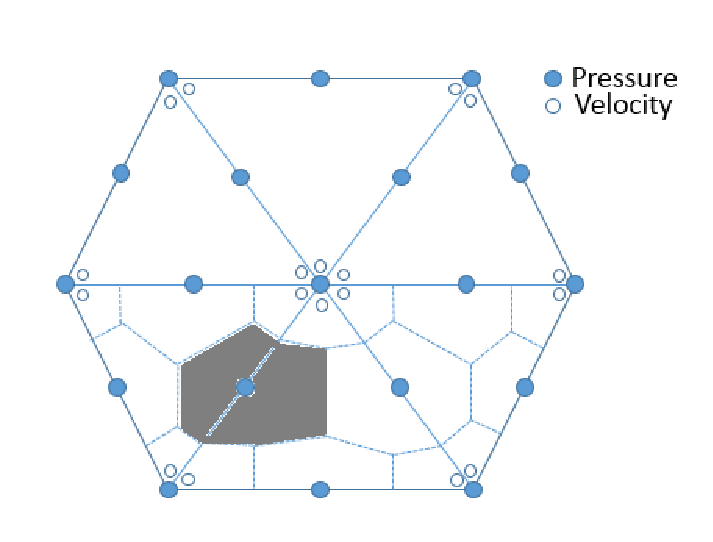
\includegraphics[width=.5\textwidth]{./Pics/P1DGP2.pdf}
\caption{2D representation of the $P_{1}DGP_{2}$ element pairs used in this work. Shaded areas denote control volumes (in which saturation field is stored), blue points represent the pressure nodes and white points the velocity nodes.}
\label{fig:fem_cv}
\end{figure}

\medskip
In the CVFE method pressure is interpollated using piecewise linear finite element basis functions, also known as shape functions, $\underline{\bf v}$ and $\underline{\bf p}$) while saturation is represented in node centered CV basis functions respectevely, and the saturation equation is solved explicitly after solving for pressure at each time.
%%%%%%%%%%%%%%%
\begin{comment}
\begin{equation}
 p^{n} = \sum_{j} \hat{p_{j}} N_{\alpha} 
\label{cvfe_pressure}
\end{equation}

\begin{equation}
 S^{n} = \sum_{j} \hat{p_{j}} M_{b} 
\label{cvfe_saturation}
\end{equation}
\end{comment}
%%%%%%%%%%%%%%%
Control volume finite element methods require high resolution meshes, as these are represented in fig.\ref{fig:fem_cv}, in regions where material properties vary abruptly, such as permeability and/or porosity contrasts at fracture-matrix interfaces. Since geometries are captured by finite elements (FE), constructed control volumes (CV) typically extend over the interfaces which may have different properties. Therefore, some average value of the permeability (defined in the FE space but projected into the CV space) is applied across the CVs at these interface. This often leads to excessive numerical dispersion especially in highly heterogeneous media. In order to overcome such artificial numerical dispersion, discontinuous hybrid finite element finite volume method (DFEFVM) was developed by \citet{nick_2011b, nick_2011a}. This novel discretisation scheme was designed to simulate flows through discrete fractured rocks in which CVs are divided along the interfaces of different materials. \citet{cumming_2011} demonstrated that CVFEM discretisation could also be used to solve Richards' equations (coupled mass conservation and Darcy equation) in heterogeneous media with relatively small computational overhead~\citep[compared with traditional coupled velocity-pressure based formulations, see also][]{cumming_phd2012}. Fluxes over CV's were calculated based upon material properties, whereas the saturation fields were volume-averaged at the interface of the materials, enforcing mass balance as described by \citet{kirkland_1992}.The conservation of mass along with Darcy's law are the governing equations while variables such as pressure, velocity,saturation and permeability define the behaviour of the flow. Finite difference methods have been applied to discretise the governing equations \citep{Luo2016,Moortgat2016,Hoteit2008} .

%\KCnote{in our case only - In conventional reservoirs the principal forces that affect fluid flow include, viscous forces, effects of gravity and permeability diffrences while in unconventional gas reservoirs flow simulation models take into account the phenomena of adsorption and diffusion \citep{abdus_2015}. Even though the mechanisms of the instabilities may vary, however it is still a function of relative mobility, gravity, viscous forces and permeability differences. All these parameters are represented under one term in the global mass balance equation.}

\medskip
The objective of this study is to investigate and accurately describe the behaviour of fingering in multiphase ($2$-phase) flows using a control volume finite element method (CVFEM). Considering the limitations of finite differences formulations the CVFE the model formulation will use a conservative computational multi-fluid porous media flow model able to exploit mesh adaptivity methods on a fully-unstructured tetrahedral grid. Also two key characteristics that describe the research concept above are: (a) the hybrid element pair $P_{n}DGP_{n+1}$ which provides discontinuous and piecewise representation for velocity and pressure fields at FE space and (b) the overlapping control volume finite element method (CVFEM)formulation.

\medskip
\KCnote{ \blue{as soon as we finish the paper}, the sections that follow include a summary of the main governing equations for multiphase compositional flow. The remainder of the paper will include a description of the viscous fingering along with the finite element method technique, a discussion of simulations results and the key conclusions. The analysis will consider ($1$)permeability heterogeities, ($2$)capturing the development of the interface and the evolution of fingers, ($3$)test-case comparison, but for now will neglect any gravitational effects.}


%%%%%%%%%%%%%%%%%%%%%%%%%%%%%%%%%%%%%%%%%%%%%%%%%%%%%%%%%%%%%%%%%%%%%%%%%%%%%%%%%%%%%%%%%%%%%%%%%%%%%%%%%%%%%%%%%%%%%%%%%%%%%%%%%%%%%%%%%%%%%%%%%%%%%%%%%%%%%%%%%%%%%%%%%%%%%%%%%%%%%%%%%%%%%%%%%%%%
\section{Governing equations and numerical scheme}\label{equations_scheme}      
Multiphase flow in porous media is described by mass conversation and Darcy equations for all the phase $\alpha$ ($\alpha$ = g, o, w, for gas, oil, and water phases). Different domains will produce different flow instabilities. In this paper, the test-cases are based on the discontinuous Galerkin (DG) method. DG-methods combine advantages of classical finite volume and finite element methods.  

%%%%%%%%%%%%%%%%%%%%%%%%%%%%%%%%%%%%%%%%%%%%%%%%%%%%%%%%%%%%%%%%%%%%%%%%%%%%%%%%%%%%%%%%%%%%%%%%%%%%%%%%%%%%%%%%%%%%%%%%%%%%%%%%%%%%%%%%%%%%%%%%%%%%%%%%%%%%%%%%%%%%%%%%%%%%%%%%%%%%%%%%%%%%%%%%%%%%
\subsection{Numerical Formulation}
\medskip

%%%%%%%%%%%%%%%
\begin{comment}
Flows in porous media are expressed by the Darcy's law and the saturation equation. At this stage the control volume finite element method is used (CVFEM). Darcy's law for immiscible multi-phase flow may be written in the form:
\begin{equation}\label{e:darcy_eq}
  \mathbf{q}_{\alpha} = -\frac{\mathcal{K}_{{r}_\alpha}\mathbf{K}}{\mu_{\alpha}}\left(\nabla p_{\alpha} - {\mathbf{s}_{u}}_{\alpha} \right),
\end{equation}
where $\mathbf{q}_{\alpha}$ is the $\alpha$-th phase Darcy velocity, $\mathbf{K}$ is the absolute permeability tensor of the porous medium, $\mathcal{K}_{{r}_\alpha}\left(S_{\alpha}\right)$ is the phase relative permeability, which is a function of the phase saturation $S_{\alpha}\left(\mathbf{r},t\right)$. $\mu_{\alpha}$, $p_{\alpha}$, $\rho_{\alpha}$, and $\mathbf{s}_{{u}_\alpha}$ are the phase dynamic viscosity, pressure, density and source term, which may include gravity and/or capillarity, respectively. 

Substituting the saturation-weighted Darcy velocity by $\mathbf{u}_\alpha= \mathbf{q}_\alpha/S_\alpha$, then Eqn.~\ref{e:darcy_eq} may be rewritten as:
\begin{equation}
  \mathbf{v}_\alpha={\underline {\underline \sigma}}_{\alpha} \mathbf{u}_{\alpha} = - \nabla p_{\alpha} + {\mathbf{s}_{u}}_{\alpha},
  \label{e:force_bal}
\end{equation}
where ${\underline {\underline \sigma}}_{\alpha}=\mu_\alpha S_\alpha \left(\mathcal{K}_{{r}_\alpha}\mathbf{K}\right)^{-1}$ represents the implicit linearisation of the viscous frictional forces. The force per unit volume $\mathbf{v}_\alpha$, defined as ${\underline {\underline \sigma}}_{\alpha} \mathbf{u}_\alpha$, is used as a prognostic variable in this approach \citep{pavlidis_2014}.

\noindent In matrix form, Eq.~\ref{e:force_bal} is: %~\ref{force-semi-disc} is: 
\begin{equation}
  {\mathbf M} \underline {\mathbf v} = -{\mathbf C} \underline{\mathbf p} + \underline {\mathbf s}_{u}, \label{force-balance-matrix-form}
\end{equation}
where $\underline{\bf v}$ and $\underline{\bf p}$ solution-vectors (also known as shape functions) are defined as:
\begin{eqnarray}
    &&\underline{{\bf v}} = \left( \left( {v_x},{v_y},{v_z} \right)_{1,1}, \left( {v_x},{v_y},{v_z} \right)  _{2,1},\ldots, \left( {v_x},{v_y},{v_z} \right)_{\mathcal{N}_\alpha,\mathcal{N}_u} \right)^{T} \;\text{and} \nonumber \\ 
    && \underline{{\bf p}} = \left(p_1, p_2, p_3, \cdots, p_{\mathcal{N}_p}\right)^T. \nonumber% \nonumber
\label{v_and_p}
\end{eqnarray}

The saturations are computed in CV space, whereas the permeability tensor $\left(\mathbf{K}\right)$ is assumed piece-wise constant in FE space. Thus the viscous-friction damping tensor $ {\underline {\underline \sigma}}_{\alpha}$ is piece-wise constant within the sub-control volumes defined through intersections between the elements and control volumes.
%Introducing a saturation-weighted Darcy velocity defined as $\mathbf{u}_\alpha= \mathbf{q}_\alpha/S_\alpha$, then Eqn.~\ref{e:darcy_eq} may be rewritten as:
%\begin{equation}
%  \mathbf{v}_\alpha={\underline {\underline \sigma}}_{\alpha} \mathbf{u}_{\alpha} = - \nabla p_{\alpha} + {\mathbf{s}_{u}}_{\alpha},
%  \label{e:force_balance}
%\end{equation}

\noindent The ${\underline {\underline \sigma}}_{\alpha}=\mu_\alpha S_\alpha \left(\mathcal{K}_{{r}_\alpha}\mathbf{K}\right)^{-1}$ represents the implicit linearisation of the viscous frictional forces. Assuming a porous media domain $\Omega\subset\mathcal{R}^{n}$ ($n$ is the number of dimensions). 
\end{comment}

%%%%%%%%%%%%%%%
\begin{comment}
The displacing and displaced fluids are considered to be incompressible and immiscible under isothermal and no source or sink conditions. In addition, we neglect the effects of capillarity and gravity in our simulations. Therefore the governing equations of conservation of mass and Darcy's law can be described below as, 

\begin{equation}
  \mathbf{q}_{\alpha} = -\frac{\mathcal{K}_{{r}_\alpha}\mathbf{K}}{\mu_{\alpha}}\left(\nabla p_{\alpha} - {\mathbf{s}_{u}}_{\alpha} \right),
\label{e:darcy_eq}
\end{equation}
where $\mathbf{q}_{\alpha}$ is the $\alpha$-th phase Darcy velocity, $\mathbf{K}$ is the absolute permeability tensor of the porous medium, $\mathcal{K}_{{r}_\alpha}\left(S_{\alpha}\right)$ is the phase relative permeability, which is a function of the phase saturation $S_{\alpha}\left(\mathbf{r},t\right)$. $\mu_{\alpha}$, $p_{\alpha}$, $\rho_{\alpha}$, and $\mathbf{s}_{{u}_\alpha}$ are the phase dynamic viscosity, pressure, density and source term, which may include gravity and/or capillarity, respectively.

\begin{equation}
  \mathbf{q}_{\alpha} = -\frac{\mathcal{K}_{{r}_\alpha}\left(S_{\alpha}\right)\mathbf{K}}{\mu_{\alpha}}\left( \nabla p_{\alpha} - {\mathbf{s}_{u}}_{\alpha} \right),
%S_{k}\left(\lambda_{k}\mathcal{K}\right)^{-1}\phi v_{\alpha} = \underline{\underline{\sigma}}_{\alpha} {\bf u}_{\alpha} = -\nabla p + \mathcal{S}_{u},
\label{E:darcy_eqn}
\end{equation}
where $\mathbf{q}_{\alpha}$ is the $k\left(\in\left\{1,N_{p}\right\}\right)$-phase Darcy flow rate. $S$, $\mathbf{K}$, $\mathcal{K}_{r\alpha}\left(S_{\alpha}\right)$ and $\mu$ are saturation, absolute permeability tensor, phase relative permeability and viscosity, respectively. $s_{u}$ is a source term (e.g., gravity force) associated with the force balance and $p$ is the pressure.

 Defining the advective velocity averaged over the entire domain -- $\mathbf{u}_{\alpha}= \mathbf{q}_{\alpha}/S_{\alpha}$, then we may rewrite Eq.(\ref{E:darcy_ext}),
\begin{equation}
  {\underline {\underline \sigma}}_{\alpha} \mathbf{u}_{\alpha} = - \nabla p + {\mathbf{s}_{u}}_{\alpha},
  \label{E:darcy_ext}
\end{equation}
$\underline{\underline{\sigma}}_{\alpha}=\mu_{\alpha}S_{\alpha}\left(\mathcal{K}_{r\alpha}\mathbf{K}\right)^{-1}$ represents the implicit linearisation of the viscous frictional forces, and is piecewise constant within each FE and is obtained via basis functions local to each CV within each element \citep{Jackson13,Radunz14}.
\end{comment}
%%%%%%%%%%%%%%%

The two-phase flow through the porous media $\Omega$ may be described by the coupled extended Darcy and global mass conservation equations,
\begin{eqnarray}
\left(\displaystyle\frac{\mu_{\alpha}S_{\alpha}}{{\mathbf K}\mathcal{K}_{r\alpha}}\right) {\mathbf u}_{\alpha} = \underline{\underline{\sigma}}_{\alpha} {\mathbf u}_{\alpha} = -\nabla p + \mathcal{S}_{u,\alpha},\;\;\; x_{i}\in\Omega, t>0 \label{eqn:darcy_eqn} \\
\phi\displaystyle\frac{\partial S_{\alpha} }{\partial t} +   \nabla \cdot \left( {\mathbf u}_{\alpha}  S_{\alpha}\right) =  \mathcal{S}_{cty,\alpha},\;\;\; x_{i}\in\Omega, t>0\label{eqn:saturation_eqn}
\end{eqnarray}
where $S$, $\mu$, ${\bf K}$, $p$ and $\phi$ are the saturation, viscosity, absolute permeability, pressure and porosity, respectively. ${\mathbf u}_{k}$ is the saturation-weighted Darcy velocity of the $k$-phase and $\mathcal{K}_{r,\alpha}$ is the relative permeability. $\mathcal{S}$ is the source term associated with the Darcy and continuity equations. $S_{\alpha}$ is saturation of the $\alpha$-phase with the constraint of $\sum\limits_{\alpha=1}^{\mathcal{N}_{p}} S_{\alpha} = 1$, where $\mathcal{N}_{p}$ denotes the number of phases.

%%%%%%%%%%%%%%%
\begin{comment}
The main equations that will be used along with the following OCVFEM techique can be summarised below. The global mass balance equation and force balance equation are solving by vanishing the velocity term and solving the system of equations for pressure. At the $n+1$ step those two equations mentioned above can be rewritten as,

\begin{equation}
M_{\sigma} {{\underline{u}}^{n+1}} = C {\underline{p}^{n+1}} + {\underline{s}_u ^{n+1}}
\label{e:mass_bal}
\end{equation}

\begin{equation}
B^T {{\underline{u}}^{n+1}} = {\underline{s}_p ^{n+1}}
\label{e:force_bal}
\end{equation}

\noindent Application of a discontinuous FEM for velocity leads to a block-diagonal $M_{\sigma}$ matrix that can be readily inverted, each block being local to an element. This system of equations can be rewritten to produce the pressure equation, 

\begin{equation}
B^T M_{\sigma} ^{-1} C{{\underline{p}}^{n+1}} = {\underline{s}_p ^{n+1}} - B^T M_{\sigma} ^{-1} {{\underline{s}}^{n+1}} 
\label{e:pressure_eq}
\end{equation}

\end{comment}
%%%%%%%%%%%%%%%

\medskip
Finite element basis functions for velocity and pressure fields are introduced in the discretisation of force-balance equation (eq.~\ref{e:darcy_eq}). Hybrid basis functions are also developed to allow CV-based velocity to be extrapolated across the entire element. $\underline{\underline{\sigma}}_{k}=\underline{\underline{\sigma}}_{k}\left({\mathbf K}, \mathcal{K}_{rk}, S_{K}, \mu_{k}\right)$ is an absorption-like term that lies in both CV and FEM spaces. Though, whilst the saturation field is calculated in CV space, permeability $\left({\mathbf K}\right)$ is piecewise constant in FE space to allow efficient representation of surface parametrised geometries. The global saturation equation (Eqn.~\ref{eqn:saturation_eqn}) is discretised in space with CV basis function and with the $\theta$-method in time as described by \citet{gomes_book_2012}. Velocities across CV interfaces (within and between elements, see fig.\ref{fig:fem_cv} below) are calculated through a directional-weighted flux-limited scheme based on upwind value of $\sigma$ at individual CV as described by \citet{jackson_2013}.

%%%%%%%%%%%%%%%%%%%%%%%%%%%%%%%%%%%%%%%%%%%%%%%%%%%%%%%%%%%%%%%%%%%%%%%%%%%%%%%%%%%%%%%%%%%%%%%%%%%%%%%%%%%%%%%%%%%%%%%%%%%%%%%%%%%%%%%%%%%%%%%%%%%%%%%%%%%%%%%%%%%%%%%%%%%%%%%%%%%%%%%%%%%%%%%%%%%%
%\section{Numerical Formulation}\label{section:NumericalFormulation}
 The method developed is applicable to $N_{p}$ fluid phases and is based on the novel family of $P_{n}(DG)-P_{m}(DG)$ element-pair consistent with the dual pressure-velocity representation in control volume (CV) and finite element (FE) spaces. These element-pairs have a discontinuous $n^{th}$-order polynomial representation for velocity and a discontinuous $m^{th}$-order of pressure. Another element pair, that can be used is the $P_{n}DGP_{m}$ with an $m^{th}$-order continuous representation for pressure. The mass balance (continuity) equations are solved in CV space and a Petrov-Galerkin finite element (FE) method is used to obtain the high-order fluxes on CV boundaries (fig.\ref{fig:fem_elem})  , which are limited to yield bounded fields.

\begin{figure}[h] 
\centering
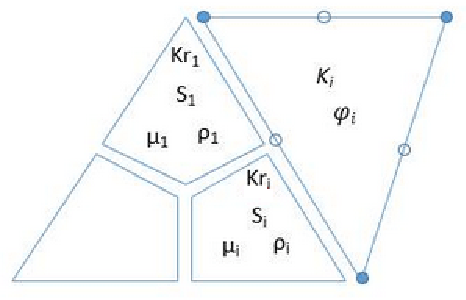
\includegraphics[width=.5\textwidth]{./Pics/element_n.pdf}
\caption{Porosity $\phi_{i}$, and permeability $K_{i}$ are associated to the elements. The velocity and pressure are associated to the element corners and the mid-points as described in fig.\ref{fig:fem_cv}; three CVs fit into a $2$D element. Saturation and saturation-dependent variables are stored CV-wise.}
\label{fig:fem_elem}
\end{figure}

Saturation, and all saturation-dependent material properties such as relative permeability and capillary pressure, are represented CV-wise. The pressure, a key difference to other CVFE methods reported previously, allows the use of CVs that do not span multiple FEs. Hence each CV (and FE) is associated with a unique set of petrophysical properties, in contrast to most previous methods in which CVs span multiple values of petrophysical properties described FE-wise.

In this model we assume that rock and fluids are incopressible thus the mass ballance for phase $\alpha$ can be written as (Eq.\ref{mass_balance})

\begin{equation}
\phi \; \frac{\partial S_{\alpha}}{\partial t} + \nabla (u_{\alpha}S_{\alpha})= \mathcal{S}_{cty,\alpha}
\label{mass_balance}
\end{equation}
 
%\noindent where $\phi$ represents the porosity, S represents the saturation and v is the saturation weighted Darcy velocity (such that $v_{\alpha}S_{\alpha}$ is the traditional Darcy velocity of phase p), and q is a volume source term, subject to the contrains on the saturation

%\begin{equation}
%\sum  S_{p}-1
%\label{saturation_constrain}
%\end{equation}

Equation \ref{mass_balance}, is discretize in time and space following the $\theta$-method. Summing over all phases and discretizing in time using the $\theta$-method yields the global mass balance equation %\ref{global_mass_balance},

\begin{eqnarray}
 && \sum_{\alpha=1}^{N_{p}} \int\limits_{\Omega_{CVi}} \; M_{i} \; \frac{\phi\left(S_{\alpha i}^{n+1}\right)-\left(S_{\alpha i}^{n}\right)}{\Delta t} dV  + \nonumber\\
 &&  \oint_{\Gamma_{CVi}} [\; \theta^{n+1/2}\; n\dot \; v_{\alpha}^{n+1}S_{\alpha}^{n+1} \; + \; (1-\theta^{n+1/2}) \; v_{\alpha}^{n}S_{\alpha}^{n}] d\Gamma \;- \nonumber\\
 &&  \int_{\Omega_{CVi}} M_{i} \; \mathcal{S}_{cty,\alpha}^{n+\theta} \; dV\; =0
\label{global_mass_balance}
\end{eqnarray}

\noindent where $\Omega_{CVi}$ and $\Gamma_{CVi}$ are the volume and boundary of CV i respectively, \textbf{n} is normal vector of the CV and $\theta$ varies smoothly between $0.5$ (corresponding to Crank-Nicolson method) and $1$ (corresponding to Backward-Euler scheme) to avoid the introduction of spurious oscillations for large grid Courant numbers. In addition to the numerical schemes above the discretised global mass and force balance equations are solved using a multigrid-like approach, see \citet{pavlidis2016}.


%%%%%%%%%%%%%%%%%%%%%%%%%%%%%%%%%%%%%%%%%%%%%%%%%%%%%%%%%%%%%%%%%%%%%%%%%%%%%%%%%%%%%%%%%%%%%%%%%%%%%%%%%%%%%%%%%%%%%%%%%%%%%%%%%%%%%%%%%%%%%%%%%%%%%%%%%%%%%%%%%%%%%%%%%%%%%%%%%%%%%%%%%%%%%%%%%%% 
\section{Brief Overview of Viscous Instabilities}\label{section:ViscousInstabilities}
\medskip
As in many areas of fluid mechanics, the behaviour of the flow for conditions that exceed critical limits may cause instabilities in the system. The flow of a fluid over or next to another heavier fluid, can produce a flow instability. Under this assumption when a fluid is injected in a porous domain saturated with an other fluid trying to displace it, viscous fingering will occur. 

\medskip
This viscous driven hydrodynamic instability results the collapse of the uniform interface between the fluids of different viscosity. This type of instability can be found across many research areas, disciplines and scales, from small chemical and medical separation systems to large scale field geological and /or reservoir systems. Starting from the work of \citet{saffman_1959} and \citet{homsy_1987}, and the experimental setup of Hele-Shaw cell by \citet{saffman_1986}, a basic mathematical model has been initially developed to describe the physics of this phenomenon. 

\medskip
In viscous fingering, a less viscous fluid (i.e. water) pushes a more viscous fluid (i.e. oil), in a thin rectangular cells (known as Hele-Shaw cells). Under the assumption that fluids remaining completely separated (or immiscible) along an interface, surface tension plays an important role in determining the shape and progress of the fingers. For homogeneous domains fingers will start to develop when surface tension acting on the interface, is opposing towards the change of shape of the interface thus the interface becomes unstable and will collapse, taking a curved shape. In heterogeneous environments this process may also be triggered by permeability differences between smaller regions. The higher the velocity of the injected fluid, the less wide (a tip-splitting behaviour) the finger will be. In addition, pressure differences (eq.\ref{eq:pressure_dif}) acting on the interface will produce a net pressure force.  

\begin{equation}
\Delta P= - \gamma \nabla \; \dot \; \hat{n} 
\label{eq:pressure_dif} 
\end{equation}

\noindent This is also know as the Young-Laplace equation, a relation describing the capillary pressure difference across the interface between two fluids. With $\Delta P$ denoting the pressure difference,$\hat{n}$ the unit normal vector out of the surface, and $\gamma$ the surface tension. As mentioned in section \ref{section:intro}, an unfavourable mobility-ratio (i.e. in a water-oil system, see eq.\ref{eq:MR}, displacement coupled with the heterogeneity of the porous medium results in viscous instability, which in turn affects the displacement efficiency of im/miscible processes. 

\begin{equation}
 MR \; = \frac{k_{rw} \; \mu_{w}}{k_{ro} \; \mu_{o}} 
\label{eq:MR}
\end{equation}

\noindent Fingering will occur in miscible displacements when the viscocity ratio is greater than unity. %As surface tension becomes weak, the front of the steady finger is susceptible to a viscous-fingering instability by the basic mechanism associated with a less viscous fluid displacing a more viscous one. After a split, each of the new lobes of the finger is stable as a result of their being thinner than the finger from which they split. 
As a result of \textit{shielding}, one of these fingers will eventually outgrow the others and will then spread to occupy the appropriate width of the cell. In the process, it reaches a width that is again unstable to splitting, and the pattern repeats. Thus, surface tension plays an essential dual role; it must be weak enough for the tip front to be unstable, but it is also the physical force causing the \textit{spreading} and ensuing repeated branching.

In  this paper, viscous instabilities for different test-cases will be investigated. Adaptive and unstructured mesh will be used to capture the collapse of the interface and the development of the fingers in relation to different values of mobility ratios and different maps of permeabilities. Initially test-cases that verify the existence of fingers in plain domain will illustrated follow by more complicated computational domains and finger patterns.  

%%%%%%%%%%%%%%%
\begin{comment}
Important parameter is the mobility (or viscosity) ratio. This is given by Eq.~\ref{eq:mobility-of-fluid} where $K$ is absolute permeability and $k_{r}$ is relative permeability :

\begin{equation}
\lambda = \frac{K\;k_{\alpha}}{\mu}
\label{eq:mobility-of-fluid}
\end{equation}

\noindent Regarding the mechanics, lets assume a porous medium, characterized by a constant permeability $K$. The flow will typically involve the displacement of a fluid of viscosity $\mu_1$  and density $\rho_1$ by a second of viscosity $\mu_2$ and density $\rho_2$. Under suitable continuum assumptions, Darcy's law, is used to describe the flow through a porous medium.

\begin{equation}
 U = \frac{b^2}{12 \mu} \nabla p
\end{equation}

and the above equation can be re-arranged for 1D steady flow as,

\begin{equation}
\frac{dp}{dx}= - \frac{\mu U}{K} + \rho g
\label{eq:pressure_dif} 
\end{equation}

where, \textit{U}, is the velocity of the more viscous fluid, \textit{b}, is the cell gap (referring to Hele-Shaw cell) and \textit{$\nabla p$} is the pressure gradient. Now consider a sharp interface or zone where density, viscosity, and solute concentration all change rapidly. Then the pressure force $(\rho_2-\rho_1)$ on the displaced fluid as a result of a virtual displacement $\delta_x$ of the interface from its simple convected location is 

\begin{equation}
\delta\rho=(\rho_2-\rho_1)=[[\frac{(\mu_1-\mu_2)U}{\kappa}]+(\rho_2-\rho_1)g] \delta\chi
\end{equation}

If the net pressure force is positive, then any small displacement will amplify, leading to an instability.In this case gravity is a stabilizing force while viscosity is destabilizing leading to critical velocity $U_c$ above which there is an instability.

\begin{equation}
U_c = \frac{(\rho_1-\rho_2) \cdot g \cdot K}{(\mu_1-\mu_2)}
\end{equation}
\end{comment}
%%%%%%%%%%%%%%%

 
%%%%%%%%%%%%%%%%%%%%%%%%%%%%%%%%%%%%%%%%%%%%%%%%%%%%%%%%%%%%%%%%%%%%%%%%%%%%%%%%%%%%%%%%%%%%%%%%%%%%%%%%%%%%%%%%%%%%%%%%%%%%%%%%%%%%%%%%%%%%%%%%%%%%%%%%%%%%%%%%%%%%%%%%%%%%%%%%%%%%%%%%%%%%%%%%%%%%

%% The Appendices part is started with the command \appendix;
%% appendix sections are then done as normal sections
%% \appendix

%% \section{}
%% \label{}

\pagebreak
\clearpage

%\listoftables
%\pagebreak
%\input{Manuscript_Table}

\pagebreak
\clearpage

%\begin{figure}[h]
%\begin{center}
%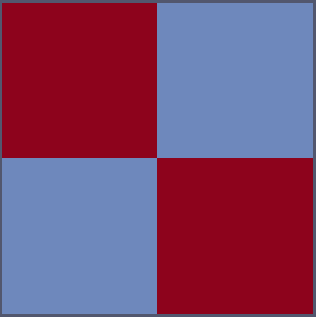
\includegraphics[width=0.75\linewidth, height=7cm]{2b2_P1DGP2_perm} 
%\caption{Caption 1}
%\label{fig:subim1}
%\end{center}

%\begin{center}
%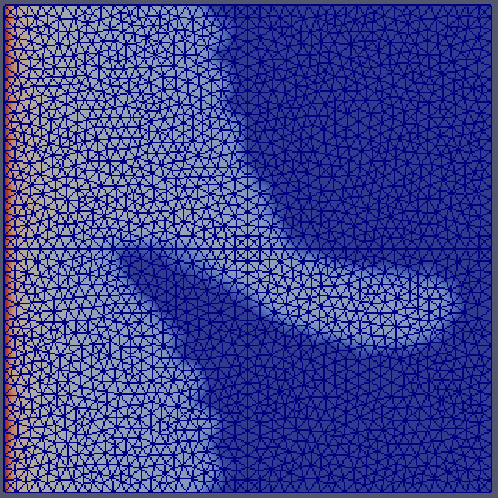
\includegraphics[width=0.75\linewidth, height=7cm]{2b2_P1DGP2_mesh} 
%\caption{Caption 1}
%\label{fig:subim1}
%\end{center}

%\begin{center}
%\centering
%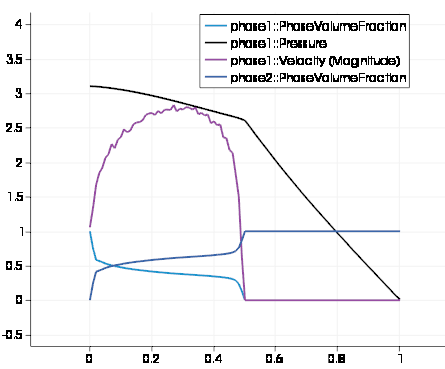
\includegraphics[width=0.75\linewidth, height=6cm]{2b2_P1DGP2_plot}
%\caption{Caption 3}
%\label{fig:subim3}
%\end{center}
 
%\caption{Caption for this figure with two images}
%\label{fig:image1}
%\end{figure}
%\pagebreak
%\clearpage

\pagebreak
\clearpage

\pagebreak
\clearpage
%
%%%%
%%%%  FIGURE 
%%%%
\begin{figure}[h]
\centering
\vbox{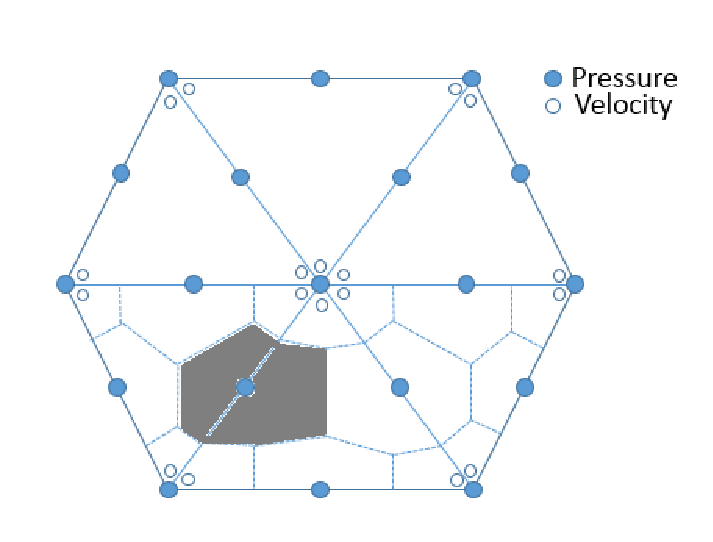
\includegraphics[width=.5\textwidth]{./Pics/P1DGP2.pdf}}
\caption{2D representation of \PN[1]{2} element pairs used in this work. Shaded areas denote control volumes across two contiguous elements. Blue and white circles represent pressure and velocity nodes, respectively.} 
\label{fig:fem_cv}
\end{figure}

\clearpage

%%%%
%%%%  FIGURE
%%%%
\begin{figure}[h]
\centering
\vbox{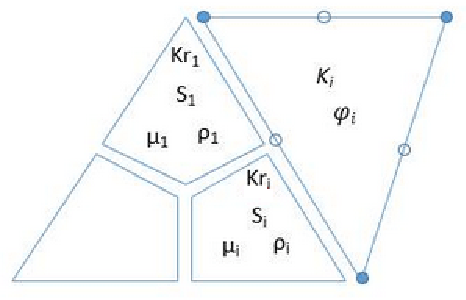
\includegraphics[width=.75\textwidth]{./Pics/element_n.pdf}}
\caption{This is a graphical representation of two different element types. Triangle {\it A} is a representation of the \PN[1]{2} element-pair, whereas triangle {\it B} represents the \PN[1]{1} element-pair. Porosity $\phi_{i}$, permeability {\bf K}$_{i}$, velocity and pressure are primarily represented in FE space whereas scalar fields (such as saturation, density, viscosity etc) are represented in CV space.}
\label{fig:fem_elem}
\end{figure}
\clearpage

%%%%
%%%%  FIGURE 
%%%%
\begin{figure}[h]
\centering
\vbox{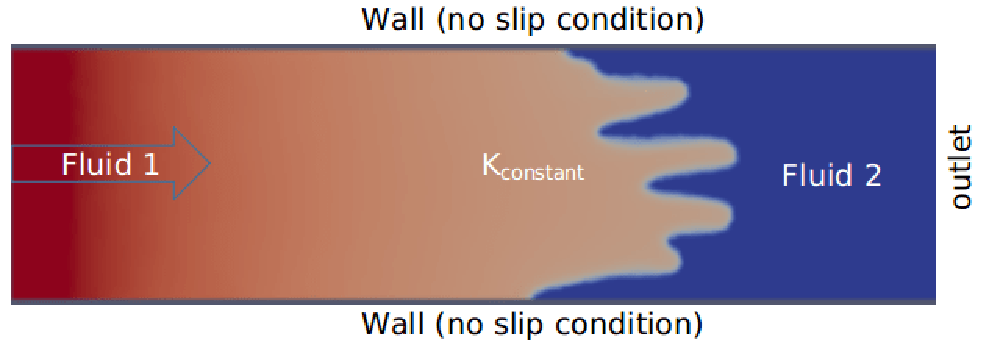
\includegraphics[width=0.75\textwidth]{./Pics/phase_vol_frac_uni_perm_1.pdf}}
\caption{Schematics of formation of flow instabilities during injection of a pure low viscosity fluid (red) into a domain saturated with a second fluid (dark blue). The ratio of viscosity between the two fluids is 5. In this case, the initially piston shape front collapses leading to the formation of several fingers.}
\label{fig:simple_case}
\end{figure}
\clearpage


%%%%
%%%%  FIGURE 
%%%%
\begin{figure}[ht] 
\vbox{
\hbox{\hspace{-0.3cm}
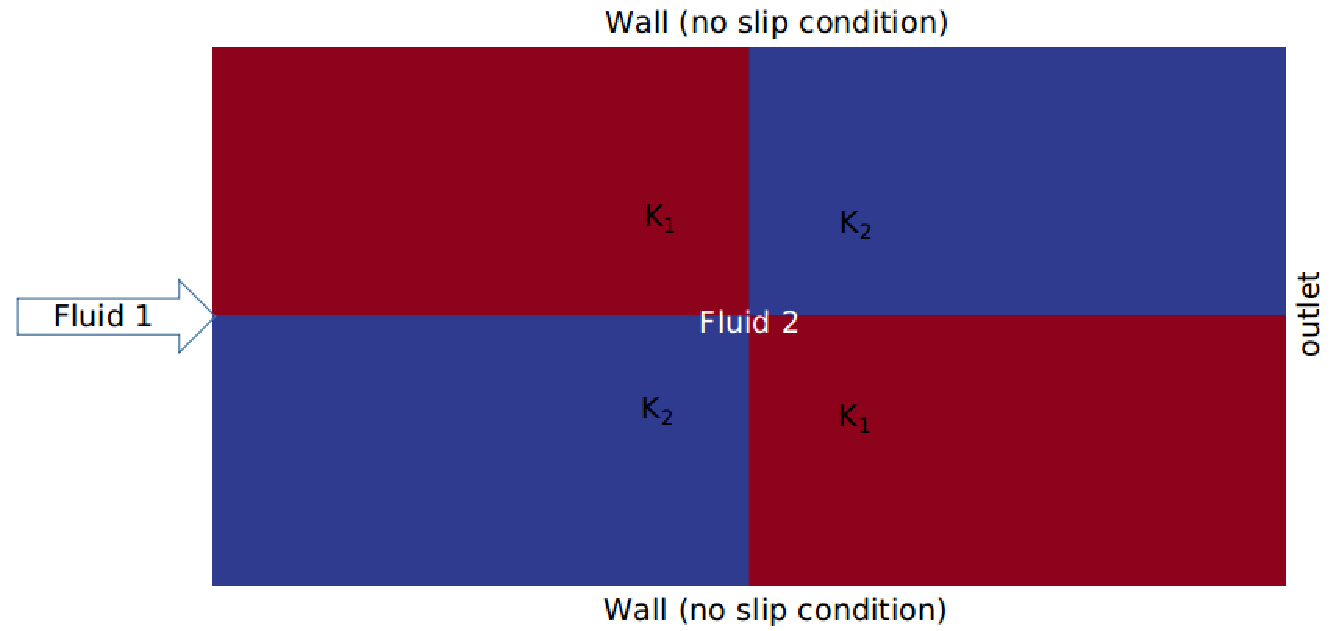
\includegraphics[width=.8\textwidth]{./Pics1/2b2_wi_fine/2b2_whole_in_fine_perm_1.pdf} 
}
\vspace{0.0cm}
\hbox{\hspace{3.5cm} (a) map of permeabilities ($\mathbf{K}$)
}
\vspace{0.25cm}
\hbox{\hspace{1.5cm}
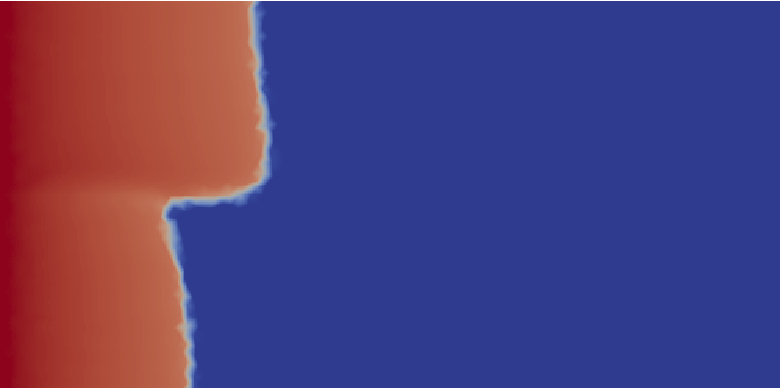
\includegraphics[width=.85\textwidth]{./Pics1/2b2_wi_fine/2b2_whole_in_fine_250_2.pdf}
}
\vspace{0.0cm}
\hbox{\hspace{4.5cm} (b) flow at t=250 
}
\vspace{0.25cm}
\hbox{\hspace{1.5cm}
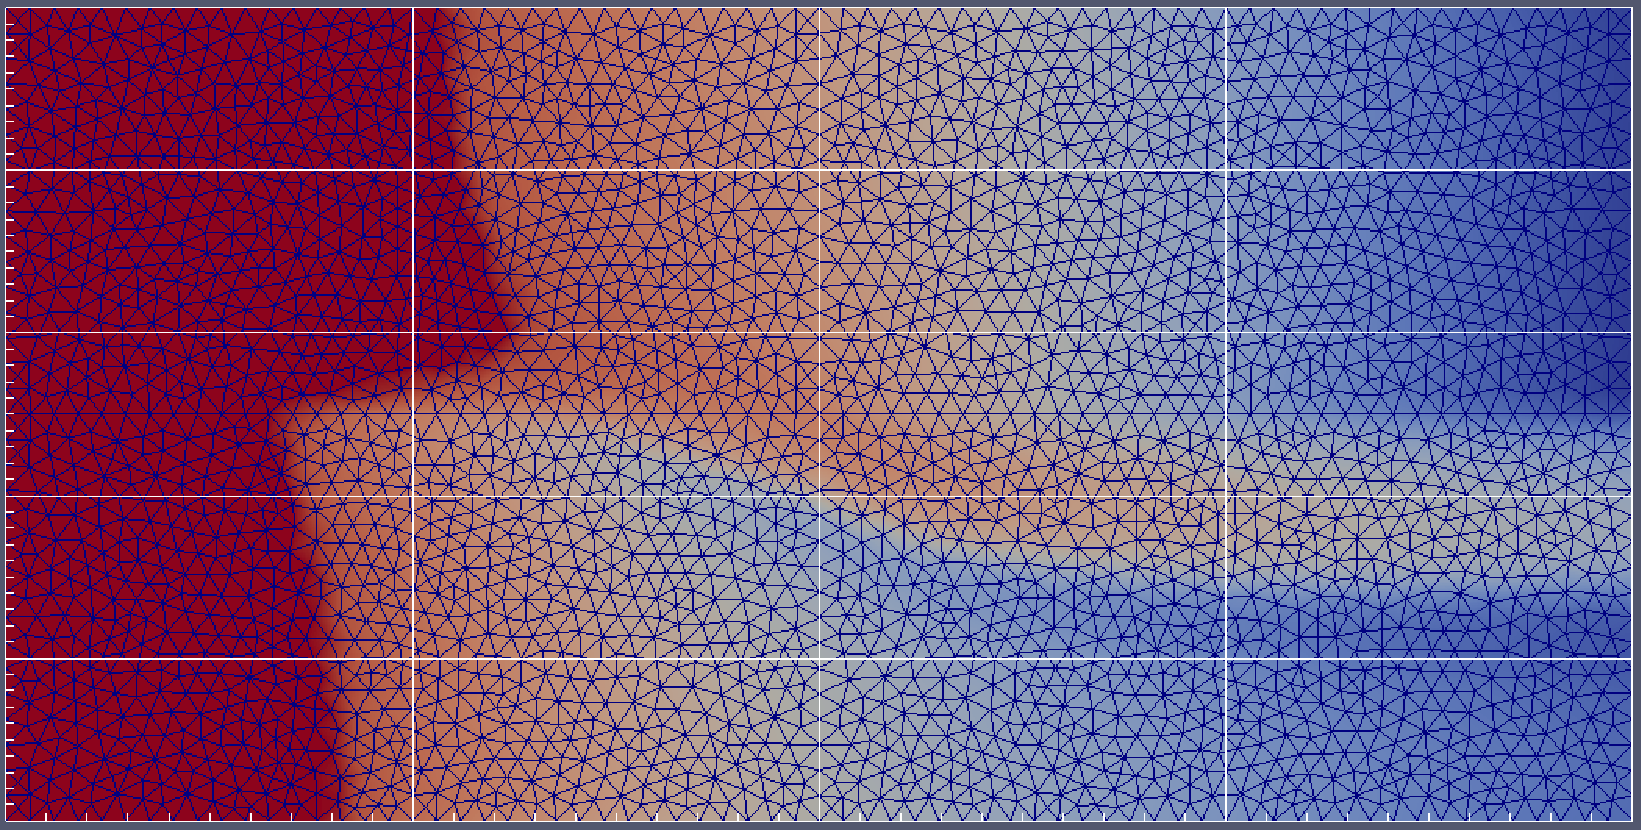
\includegraphics[width=.65\textwidth]{./Pics1/2b2_wi_fine/2b2_whole_in_fine_3000_2.pdf}
}
\vspace{0.0cm}
\hbox{\hspace{4.0cm} (c) flow at t=3000   
}}     
\caption{Model validation of fluid displacement in heterogeneous porous media ({\it VR}=1): (a) the domain is divided into four subdomains with prescribed synthetic permeability, $\mathbf{K}_{1}=1$ and $\mathbf{K}_{2}=2.5$; (b-c) snapshots of saturation (displacing fluid) field at t=$25$s and t=$300$ sec. The domain is discretised with $5960$ \PN[1]{2} elements. }
\label{fem_cv_represent_a}
\end{figure}
\clearpage



%%%%
%%%%  FIGURE
%%%%
\begin{landscape}
\begin{figure}[ht] 
\vbox{\vspace{-1cm}
\hbox{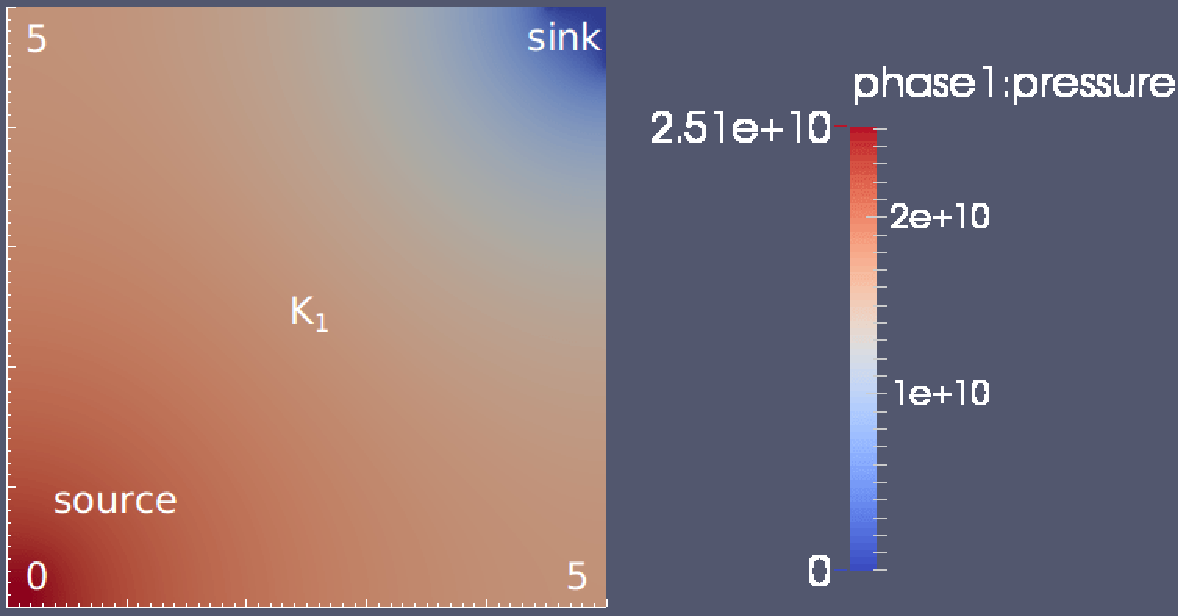
\includegraphics[width=.7\textwidth]{./Pics1/Saffman_homogeneous_MR3/saffman_homo_fixed_2.pdf}
      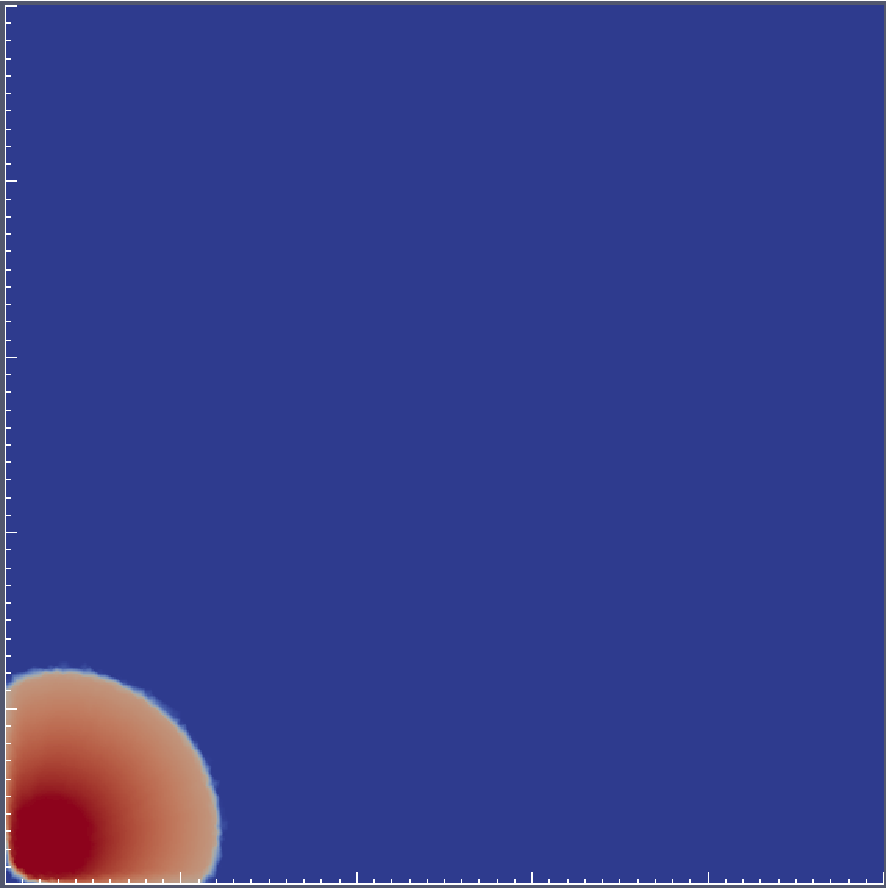
\includegraphics[width=.37\textwidth]{./Pics1/Saffman_homogeneous_MR3/saffman_homo_fixed_250.pdf}
      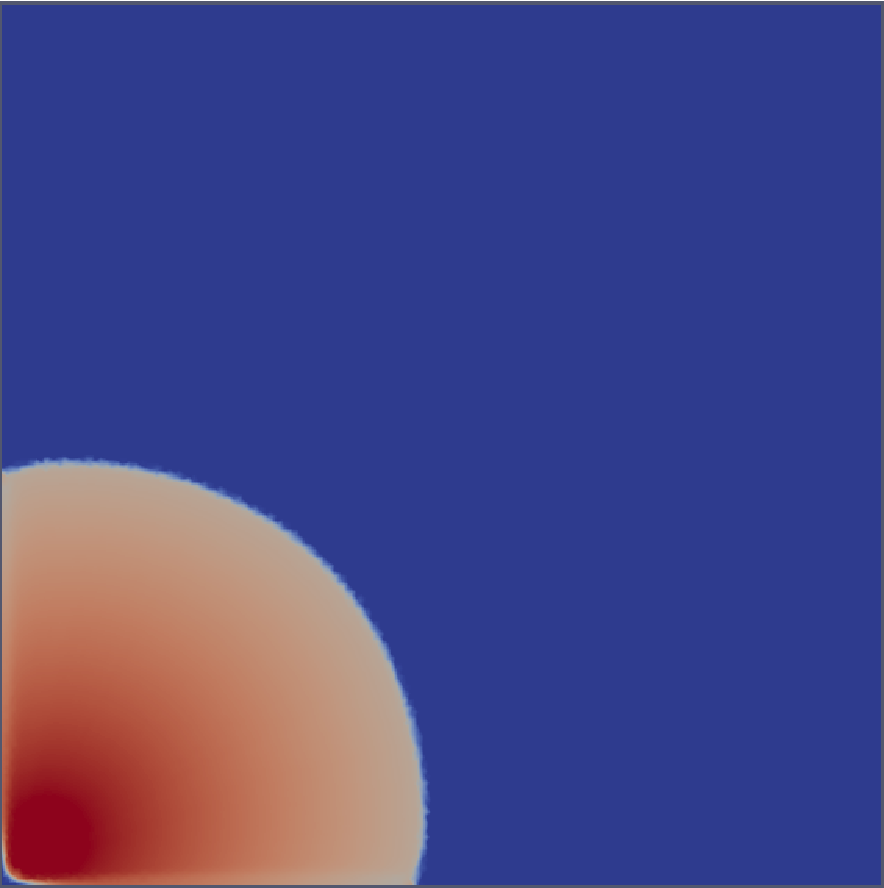
\includegraphics[width=.37\textwidth]{./Pics1/Saffman_homogeneous_MR3/saffman_homo_fixed_1000.pdf}}
\vspace{0.cm}
\hbox{\hspace{2.5cm} (a) pressure at t=0s \hspace{5.cm} (b) t=0.87s \hspace{2.75cm} (c) t=3.54s}
\vspace{0.5cm}
\hbox{
      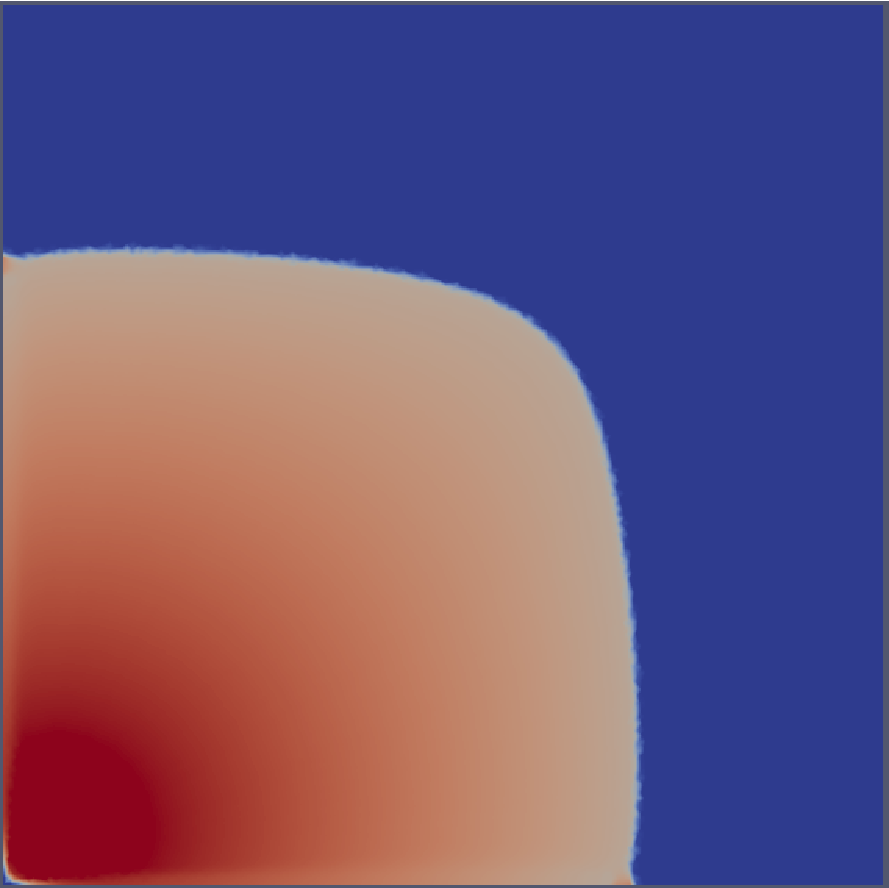
\includegraphics[width=.375\textwidth]{./Pics1/Saffman_homogeneous_MR3/saffman_homo_fixed_2500.pdf}
      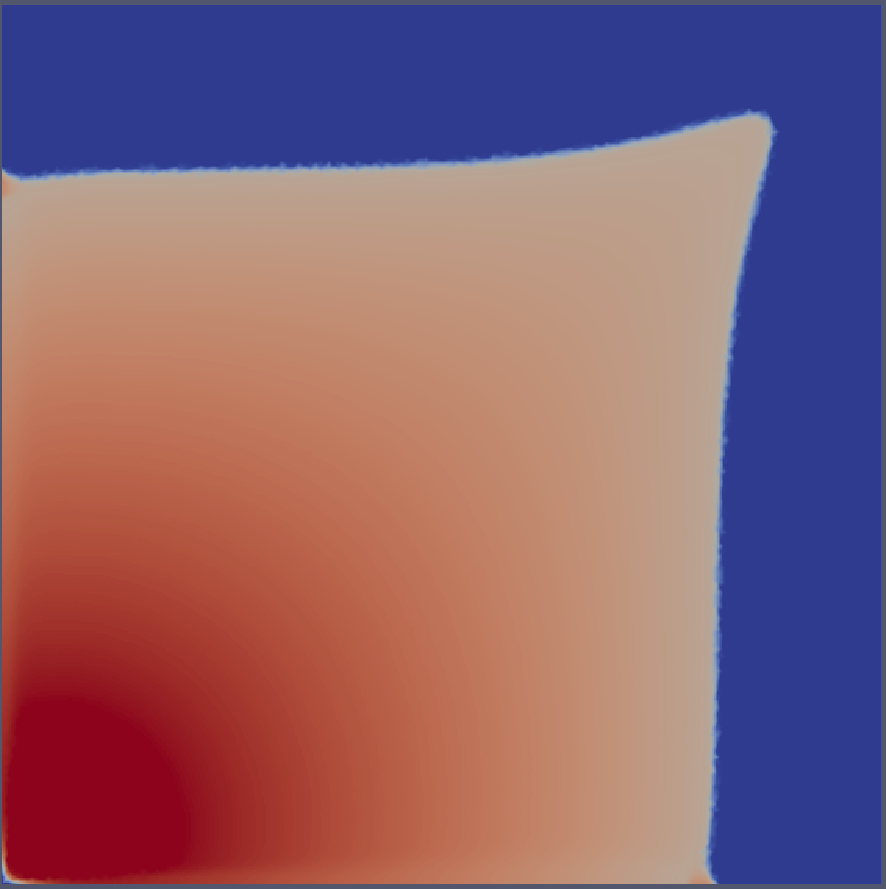
\includegraphics[width=.375\textwidth]{./Pics1/Saffman_homogeneous_MR3/saffman_homo_fixed_3500.pdf} 
      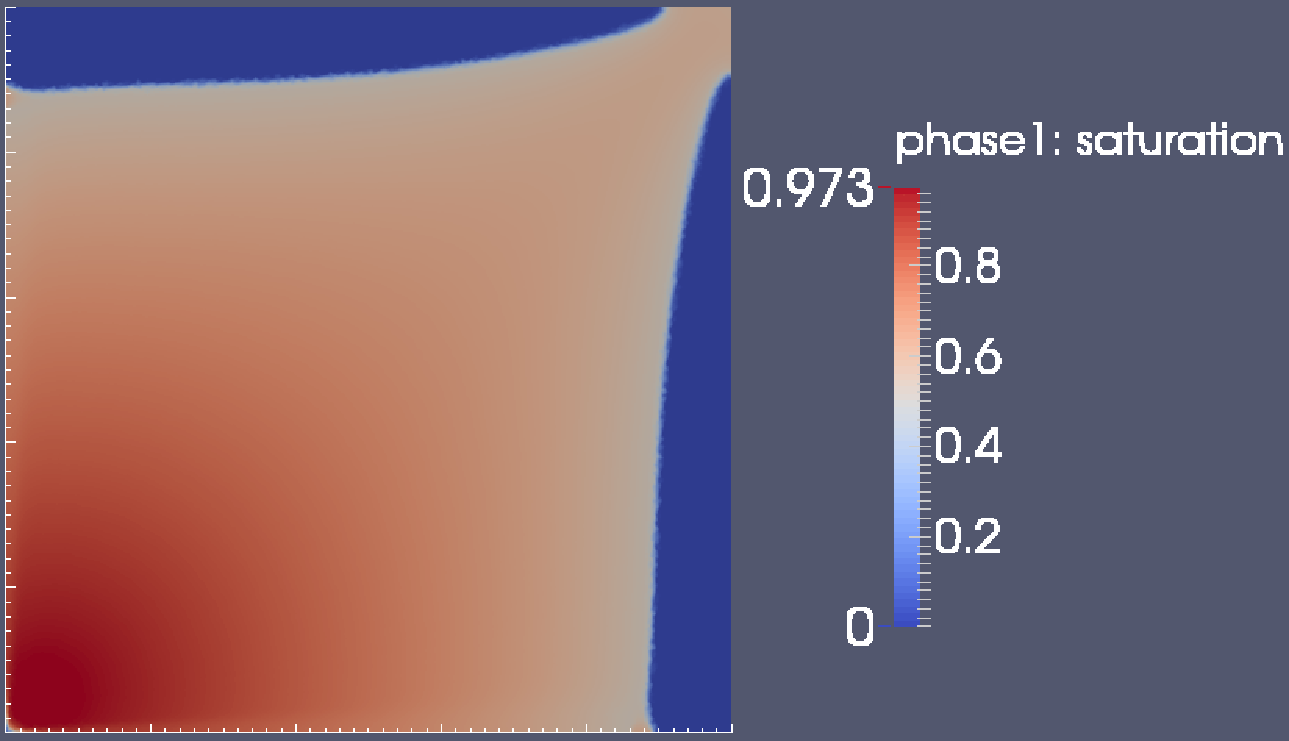
\includegraphics[width=.65\textwidth]{./Pics1/Saffman_homogeneous_MR3/saffman_homo_fixed_end.pdf}}
\vspace{0.cm}
\hbox{ \hspace{1.cm} (d) t=8.86s \hspace{3.0cm} (e) t=12.41s   \hspace{4.0cm} (f) t=17.95s}
\vspace{0.cm}
}   
\caption{Simulated flow in a Hele-Shaw cell ({\it VR}=3): (a) initial pressure profile $\left(\text{in g.cm}^{-1}\text{.s}^{-2}\right)$ with source and sink regions are explicitly shown along with dimensions (in cm); (b-f) snapshots of wetting phase saturation showing flow profile as the simulation evolves. The domain contains $47500$ \PN[1]{2} triangular elements.}
\label{fig:homoheleshaw_VN3}
\end{figure}
\end{landscape}
\clearpage



%%%%
%%%%  FIGURE
%%%%
\begin{landscape}
\begin{figure}[ht] 
\vbox{\vspace{-1cm}
\hbox{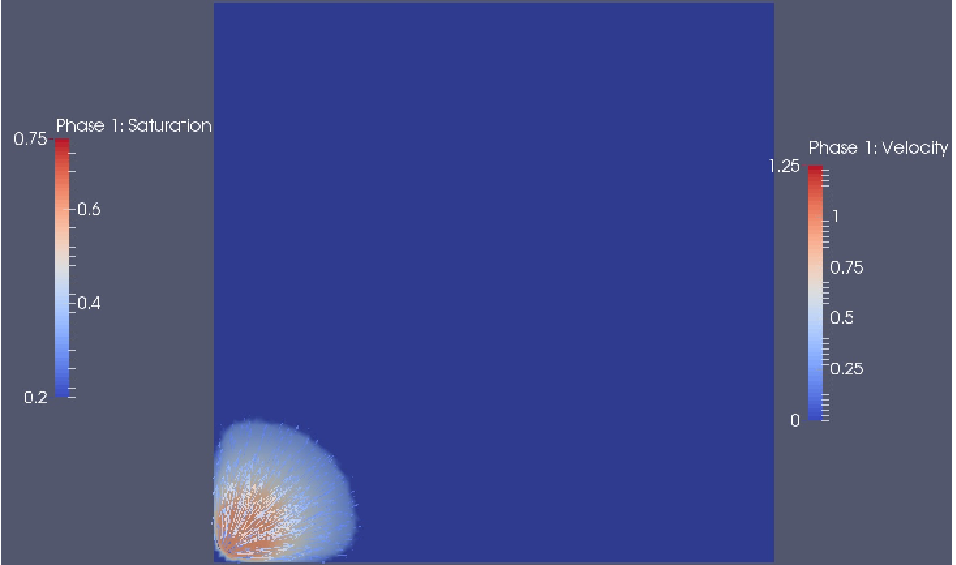
\includegraphics[width=.9\textwidth, height=0.5\textwidth]{./Pics1/Saffman_homogeneous_VR10/ST_Homog_VR10_D201c.pdf}
\hspace{0.5cm}      
      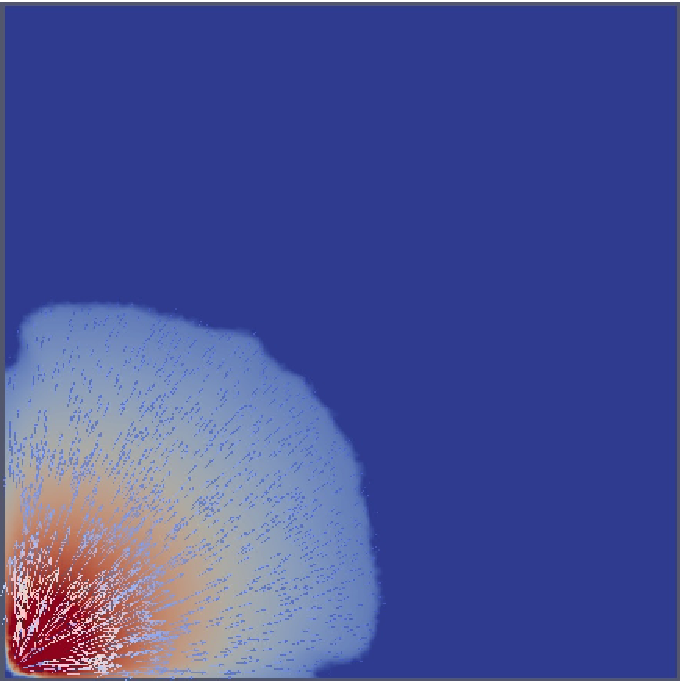
\includegraphics[width=.5\textwidth]{./Pics1/Saffman_homogeneous_VR10/ST_Homog_VR10_D1001c.pdf}}
\vspace{0.cm}
\hbox{\hspace{5.cm} (a) t=0.66s \hspace{8.cm} (b) t=3.43s }
\vspace{0.5cm}
\hbox{
      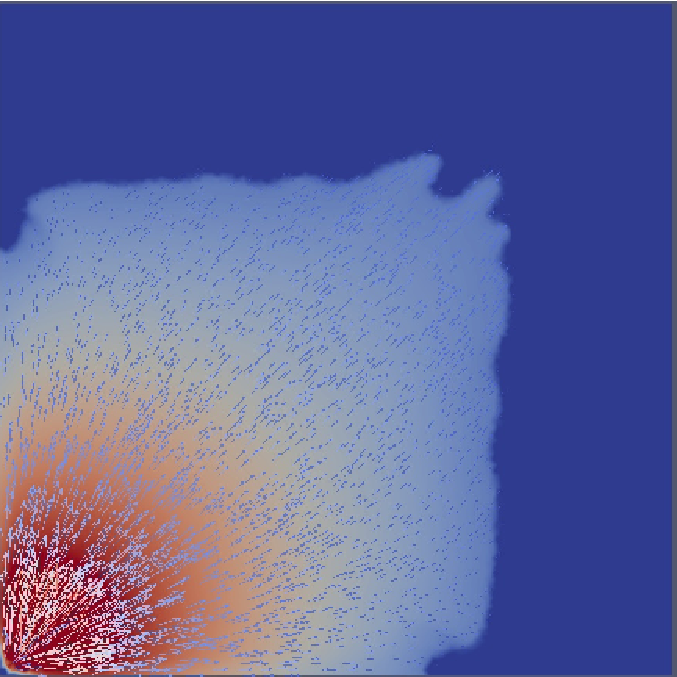
\includegraphics[width=.5\textwidth]{./Pics1/Saffman_homogeneous_VR10/ST_Homog_VR10_D2001c}
      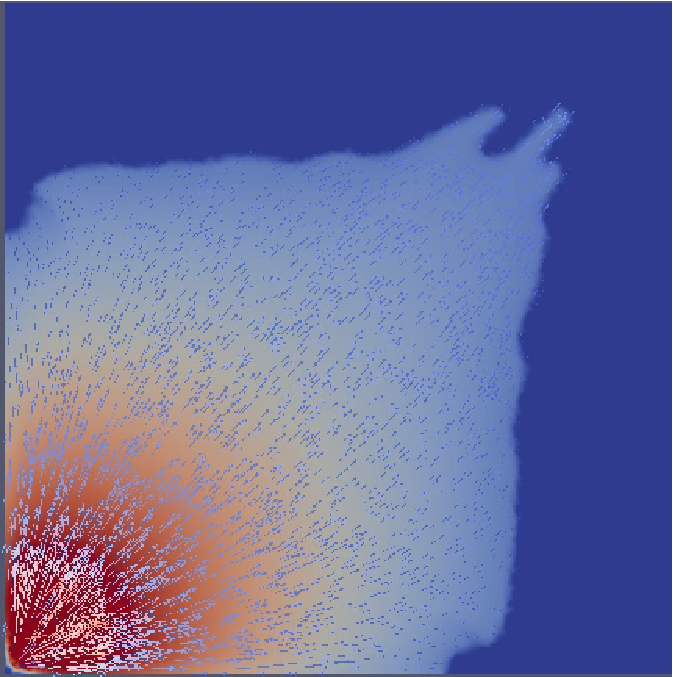
\includegraphics[width=.5\textwidth]{./Pics1/Saffman_homogeneous_VR10/ST_Homog_VR10_D2201c}
      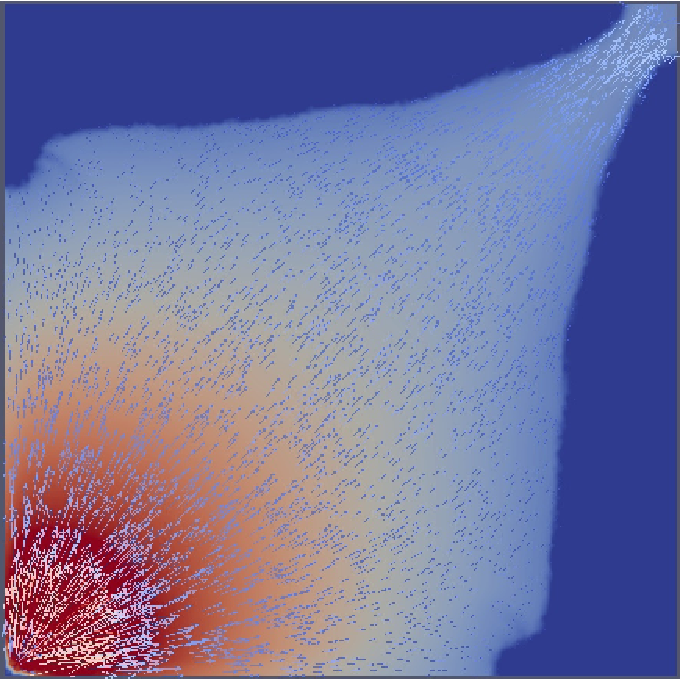
\includegraphics[width=.5\textwidth]{./Pics1/Saffman_homogeneous_VR10/ST_Homog_VR10_D3001c}}
\vspace{0.cm}
\hbox{ \hspace{2.cm} (c) t=6.92s \hspace{4.5cm} (d) t=7.61s \hspace{4.5cm} (e)t=10.00s}
\vspace{0.cm}
}   
\caption{Simulated flow in a Hele-Shaw cell ({\it VR}=10): snapshots of overlapped wetting phase saturation and velocity vectors showing flow profile as the simulation evolves. The domain contains $26313$ \PN[1]{2} triangular elements.}
\label{fig:homoheleshaw_VN10}
\end{figure}
\end{landscape}
\clearpage

%%%%
%%%%  FIGURE
%%%%
\begin{landscape}
\begin{figure}[ht] 
\vbox{\vspace{-1cm}
\hbox{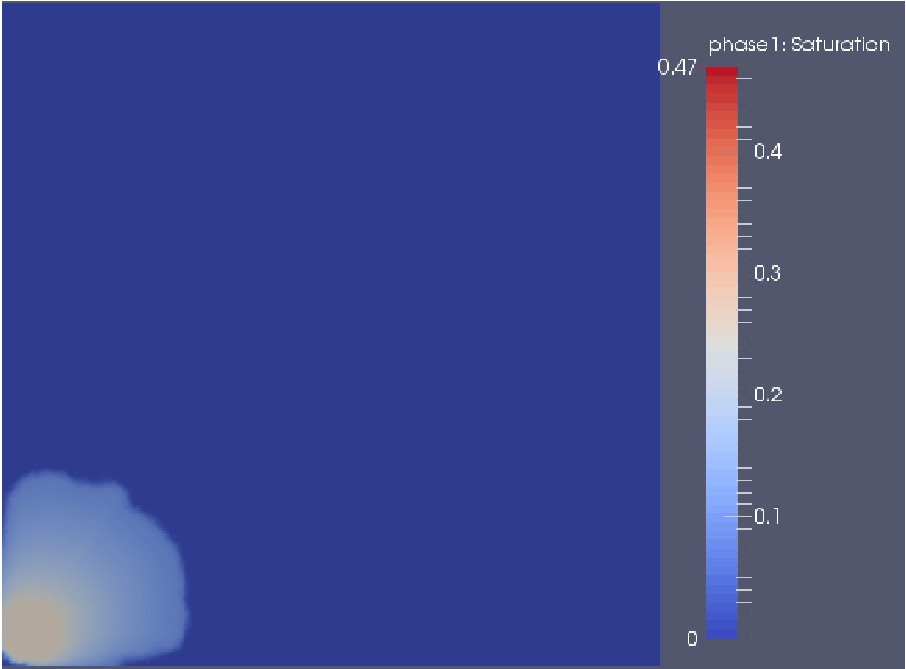
\includegraphics[width=.9\textwidth, height=0.5\textwidth]{./Pics1/Saffman_homogeneous_VR150/ST_Homog_VR150_D300b}
\hspace{0.5cm}      
      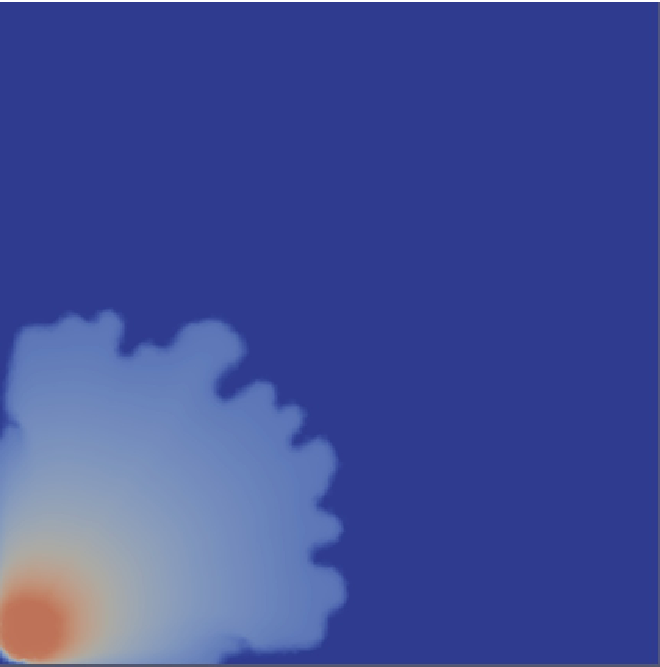
\includegraphics[width=.5\textwidth]{./Pics1/Saffman_homogeneous_VR150/ST_Homog_VR150_D1600b}}
\vspace{0.cm}
\hbox{\hspace{5.cm} (a) t=0.27s \hspace{8.cm} (b) t=0.94s }
\vspace{0.5cm}
\hbox{
      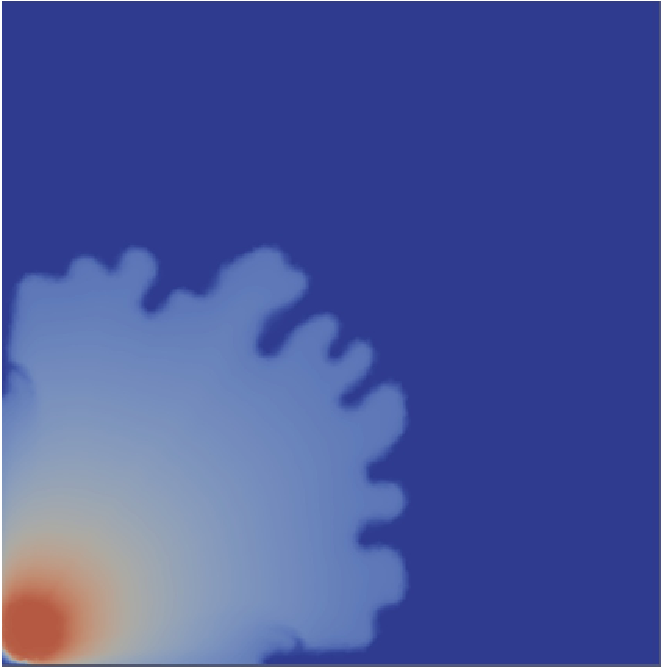
\includegraphics[width=.5\textwidth]{./Pics1/Saffman_homogeneous_VR150/ST_Homog_VR150_D2700b}
      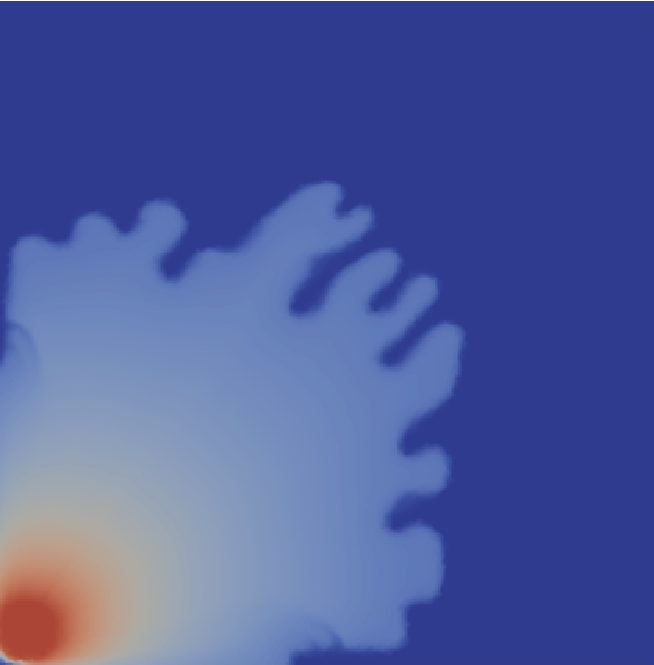
\includegraphics[width=.5\textwidth]{./Pics1/Saffman_homogeneous_VR150/ST_Homog_VR150_D4000b}
      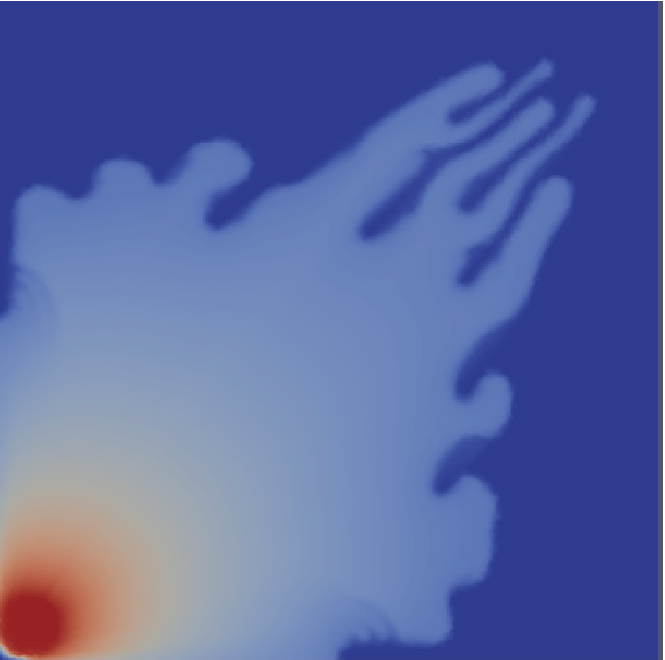
\includegraphics[width=.5\textwidth]{./Pics1/Saffman_homogeneous_VR150/ST_Homog_VR150_D7000b}}
\vspace{0.cm}
\hbox{ \hspace{2.cm} (c) t=1.32s \hspace{4.5cm} (d) t=1.70s \hspace{4.5cm} (e)t=2.31s}
\vspace{0.cm}
}   
\caption{Simulated flow in a Hele-Shaw cell ({\it VR}=150): snapshots of wetting phase saturation showing flow profile as the simulation evolves. The domain contains $26313$ \PN[1]{2} triangular elements.}
\label{fig:homoheleshaw_VN10}
\end{figure}
\end{landscape}
\clearpage


%%%%
%%%%  FIGURE
%%%%
\begin{landscape}
\begin{figure}[ht] 
\hbox{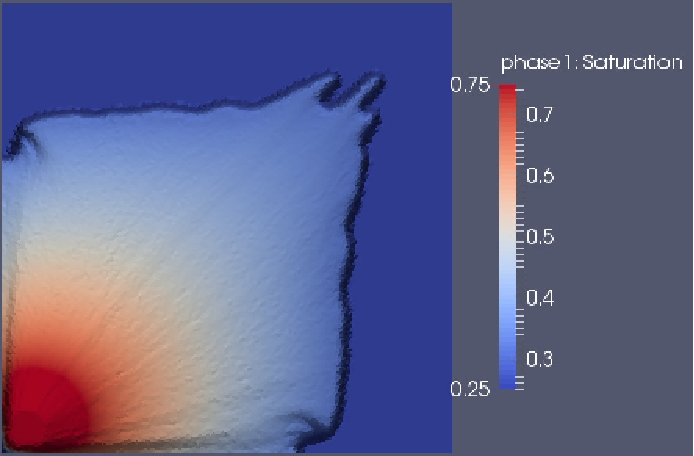
\includegraphics[width=.5\textwidth]{./Pics1/Saffman_homogeneous_VR10/ST_Homog_VR10_D2201_bbd}
       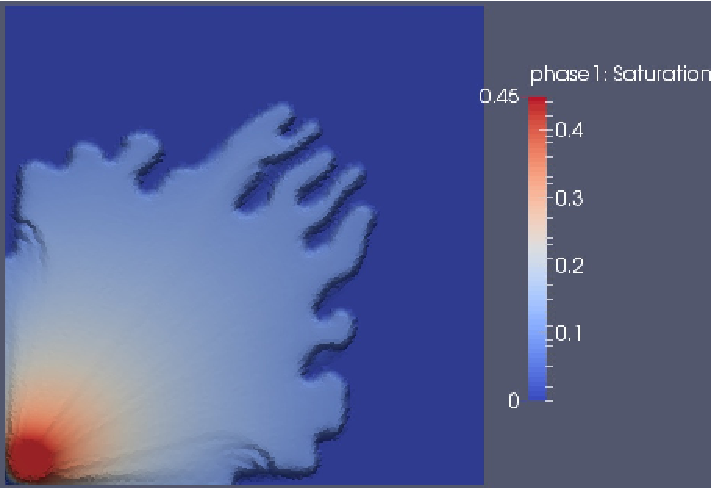
\includegraphics[width=.49\textwidth]{./Pics1/Saffman_homogeneous_VR150/ST_Homog_VR150_D5003_k2b}}
\caption{Simulated flow in Hele-Shaw cells performed with viscosity ratios of 10 (left, t=7.61s) and 150 (t=1.94s). Width of largest fingers are approximetely 0.70 and 0.90cm, which are in good agreement with values obtained from \citet{guan_2003}'s analytic solution. Domains of both simulations contain $26313$ \PN[1]{2} triangular elements.\red{(More pics to be added!!)}}
\label{fig:homoheleshaw_VN10_VN150}
\end{figure}
\end{landscape}



\begin{comment}

%%%%
%%%%  FIGURE
%%%%
\begin{landscape}
\begin{figure}[ht] 
\vbox{\vspace{-1cm}
\hbox{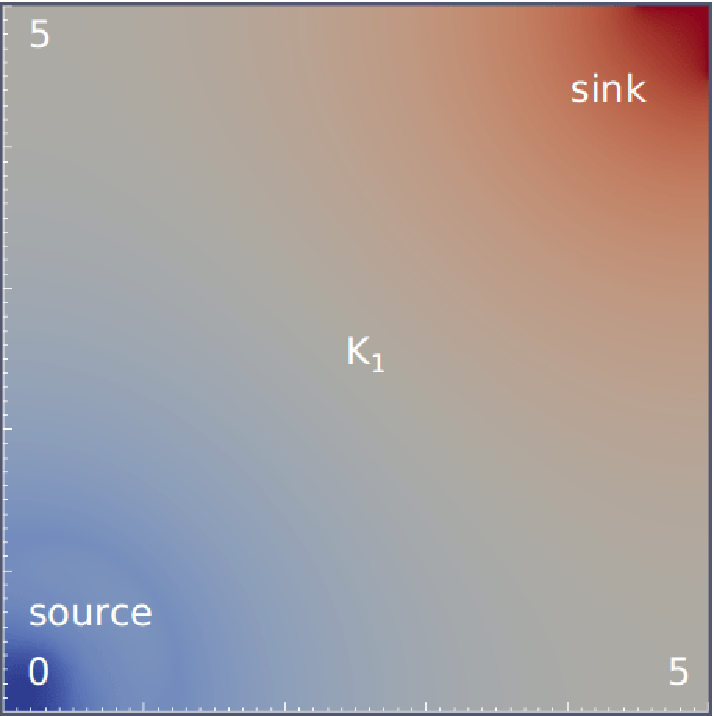
\includegraphics[width=.5\textwidth]{./Pics1/Saffman_homogeneous/saffman_homo_fixed_1.pdf}
      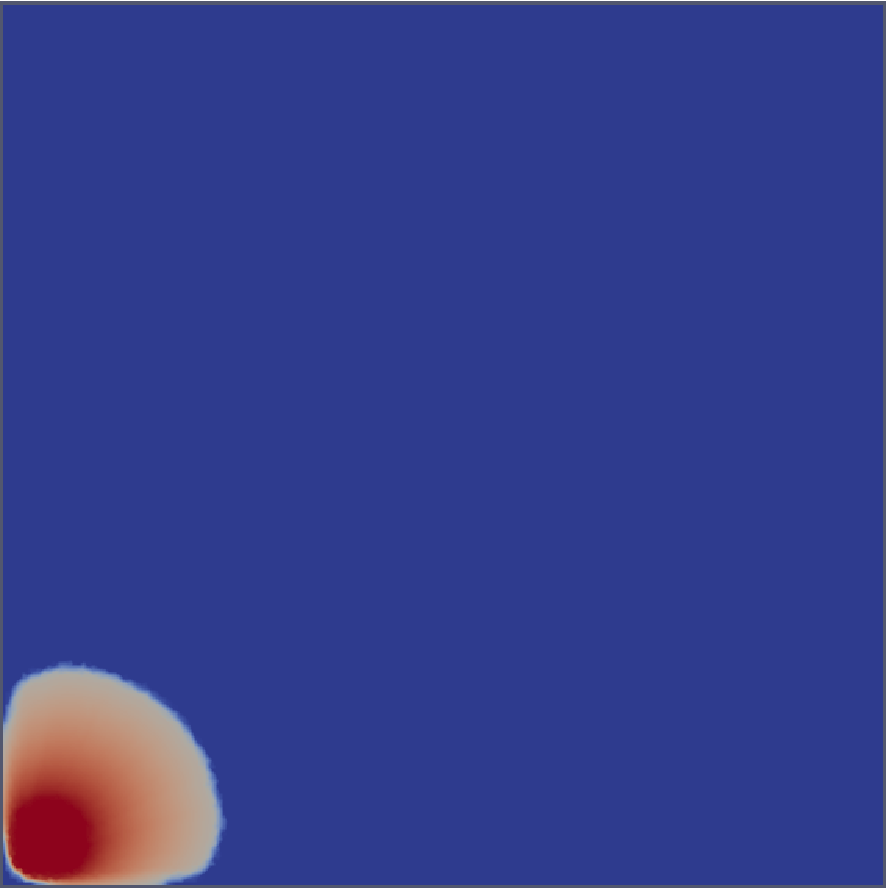
\includegraphics[width=.5\textwidth]{./Pics1/Saffman_homogeneous/saffman_homo_fixed_250_1.pdf}
      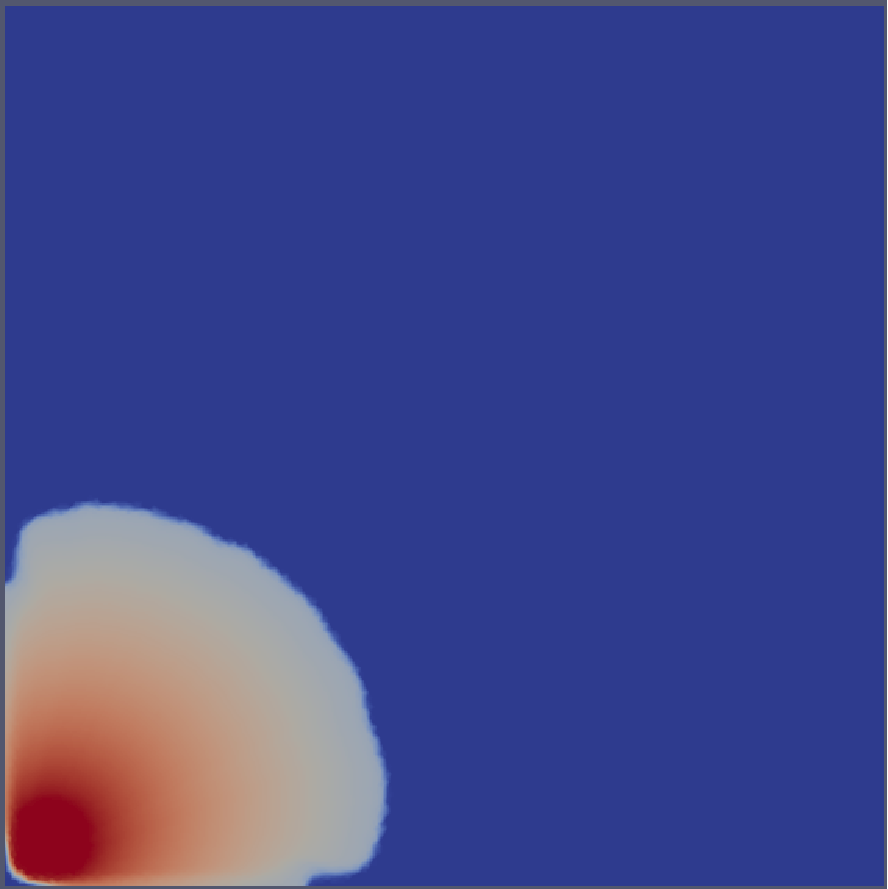
\includegraphics[width=.5\textwidth]{./Pics1/Saffman_homogeneous/saffman_homo_fixed_1000.pdf}}
\vspace{0.cm}
\hbox{\hspace{1.0cm} (a) pressure at t=0 \hspace{3.cm} (b) t=250\red{(???)} \hspace{3.0cm} (c) t=1000\red{(???)}}
\vspace{0.5cm}
\hbox{
      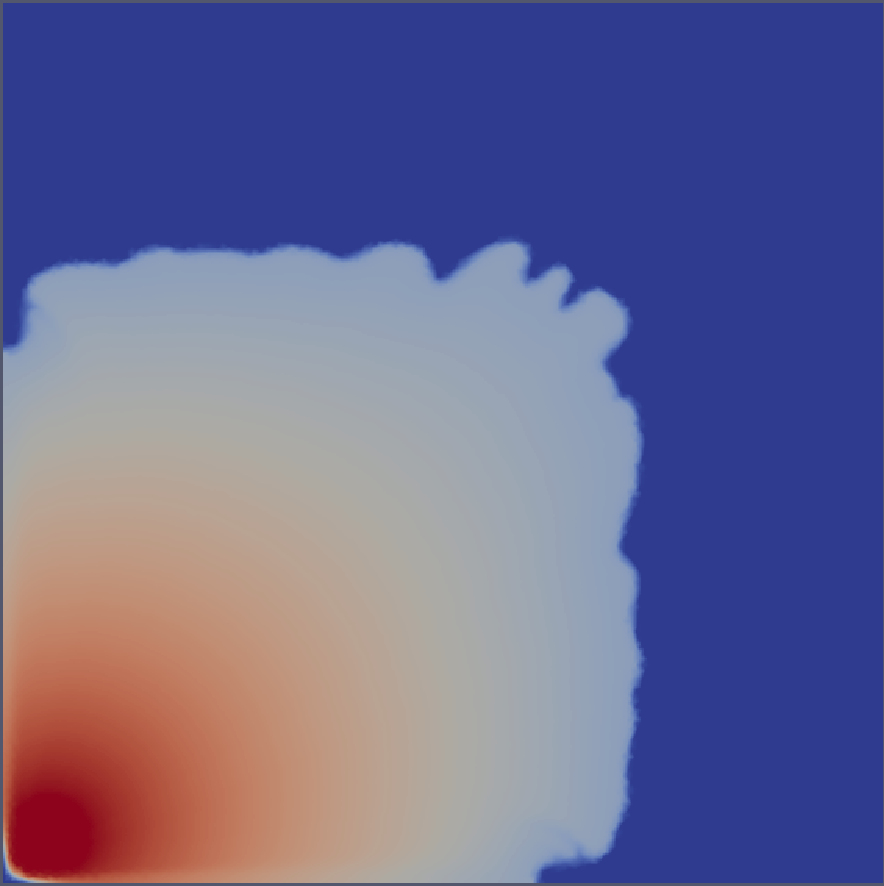
\includegraphics[width=.5\textwidth]{./Pics1/Saffman_homogeneous/saffman_homo_fixed_6000.pdf}
      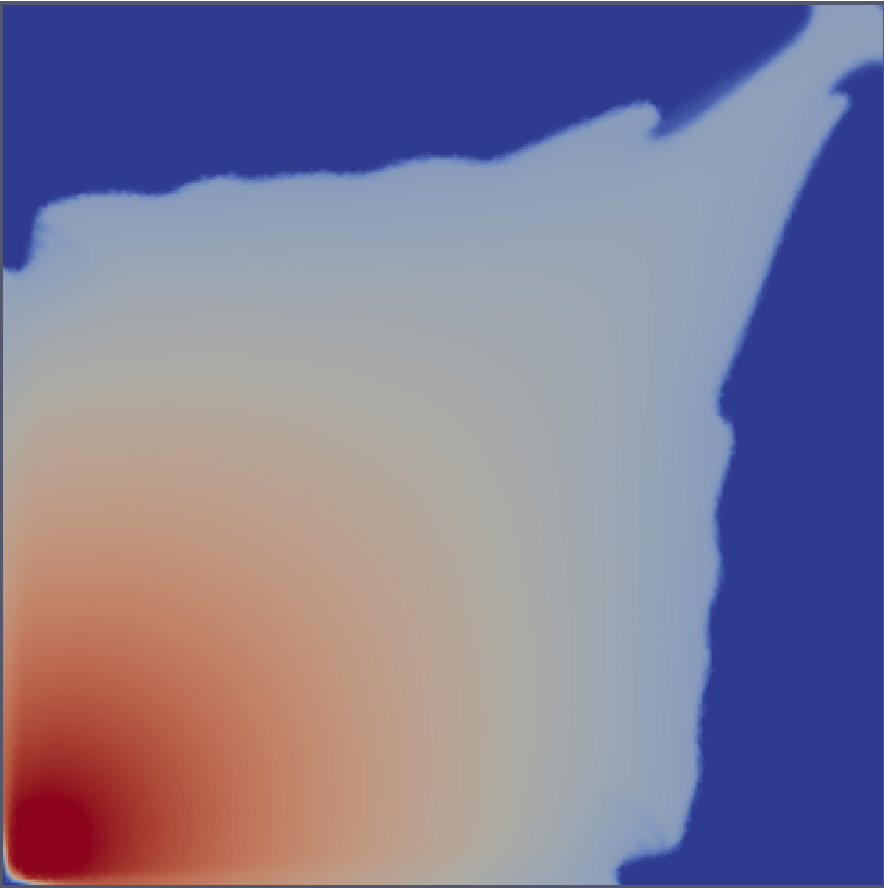
\includegraphics[width=.5\textwidth]{./Pics1/Saffman_homogeneous/saffman_homo_fixed_end_1.pdf}}
\vspace{0.cm}
\hbox{ \hspace{2.cm} (d) t=6000\red{(???)} \hspace{3.cm} (e) t=XXX\red{(???)}}
\vspace{0.cm}
}   
\caption{Simulated flow in a Hele-Shaw cell ({\it VR}=10): (a) pressure profile $\left(\text{in g.cm}^{-1}\text{.s}^{-2}\right)$ with source and sink regions explicitly shown along with dimensions (in cm); (b-e) snapshots of wetting phase saturation showing flow profile as the simulation evolves. The domain contains $47000$ \PN[1]{2} triangular elements. The pressure and saturation range of values are the same like the  case in fig.\ref{fig:homoheleshaw_VN3}.}
\label{fig:homoheleshaw_VN10}
\end{figure}
\end{landscape}
\clearpage
\end{comment}


%%%
%%% FIGURE XXXXXX
%%%
\begin{landscape}
  \begin{figure}[ht]
  \vbox{\vspace{-1cm}
      \hbox{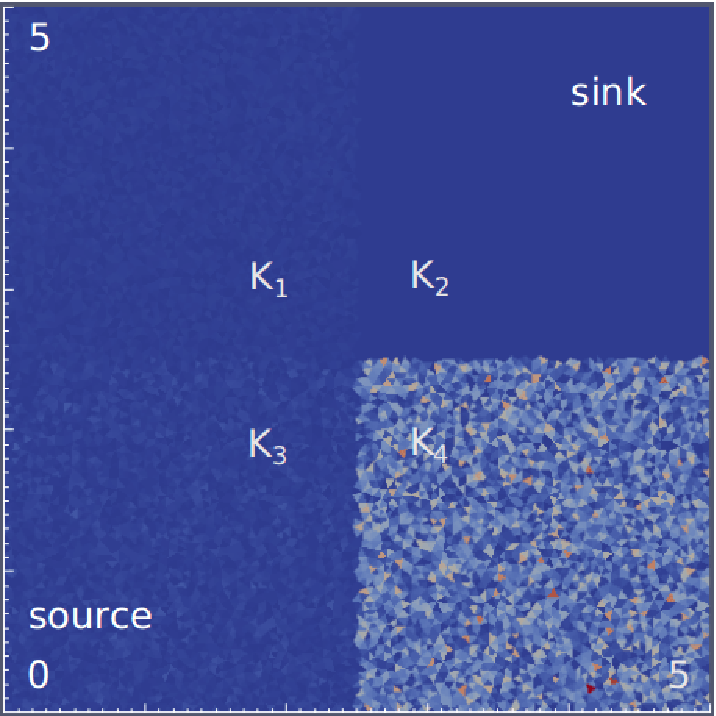
\includegraphics[width=.5\textwidth]{./Pics1/Saffman_heterogeneous/saffman_heter_fixed_1.pdf}
            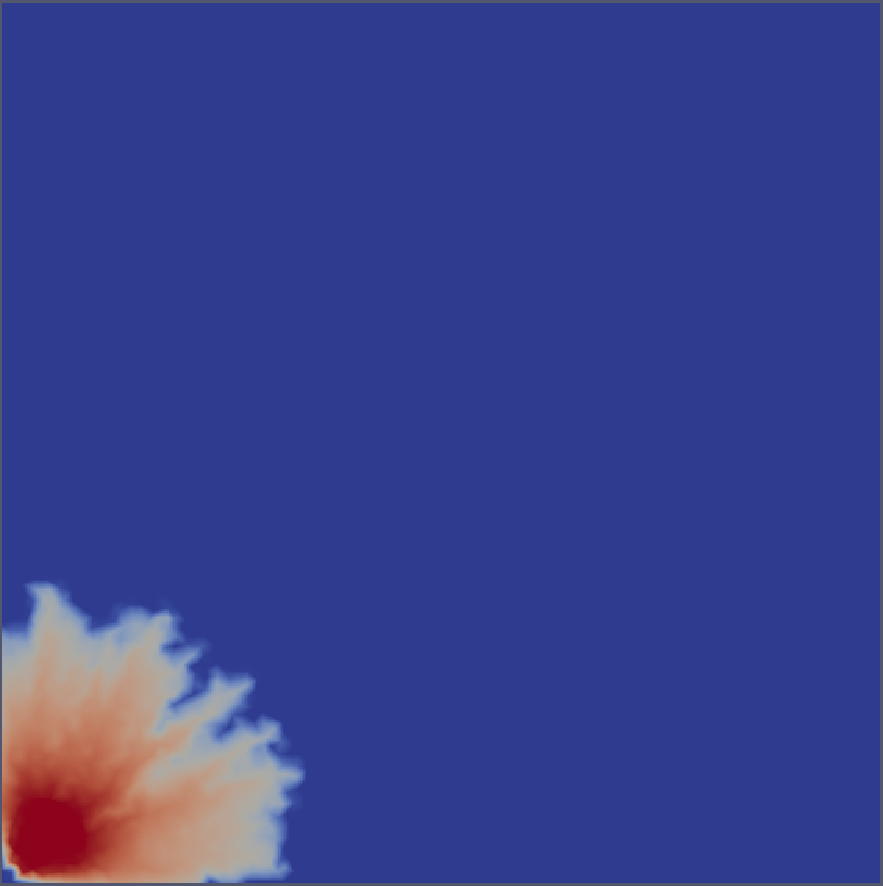
\includegraphics[width=.5\textwidth]{./Pics1/Saffman_heterogeneous/saffman_heter_fixed_500.pdf} 
            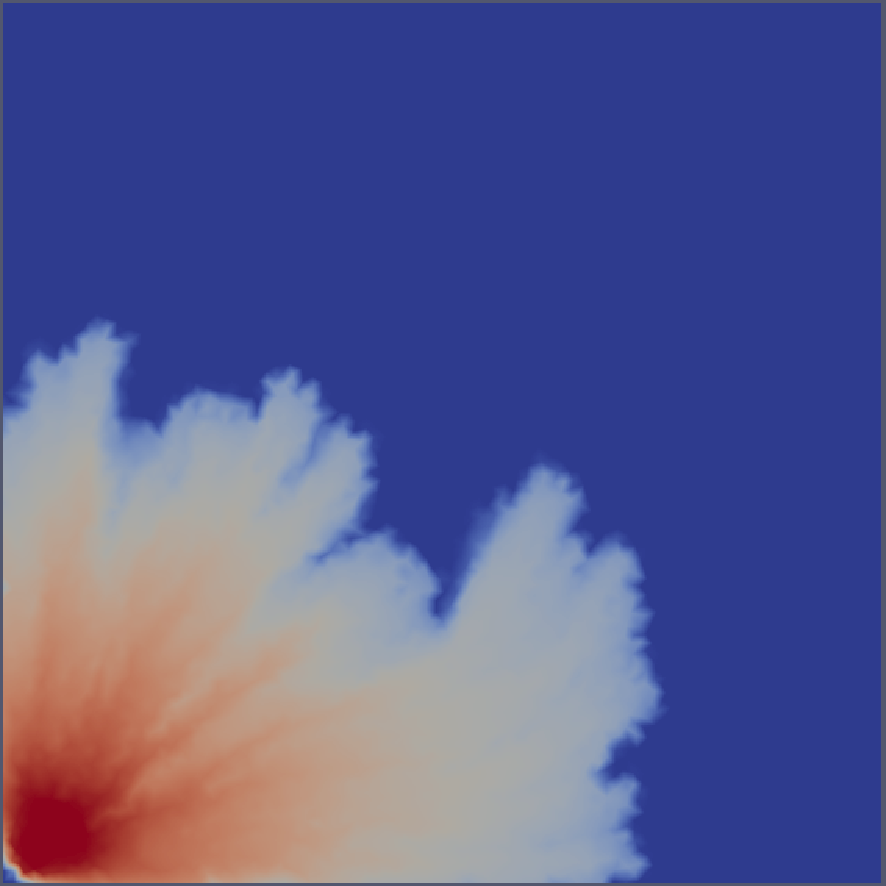
\includegraphics[width=.5\textwidth]{./Pics1/Saffman_heterogeneous/saffman_heter_fixed_2000.pdf} }
      \hbox{\hspace{1.0cm} (a) permeability map \hspace{3.cm} (b) t=0.75s \hspace{4.0cm} (c) t=8s}
      \vspace{0.5cm}
      \hbox{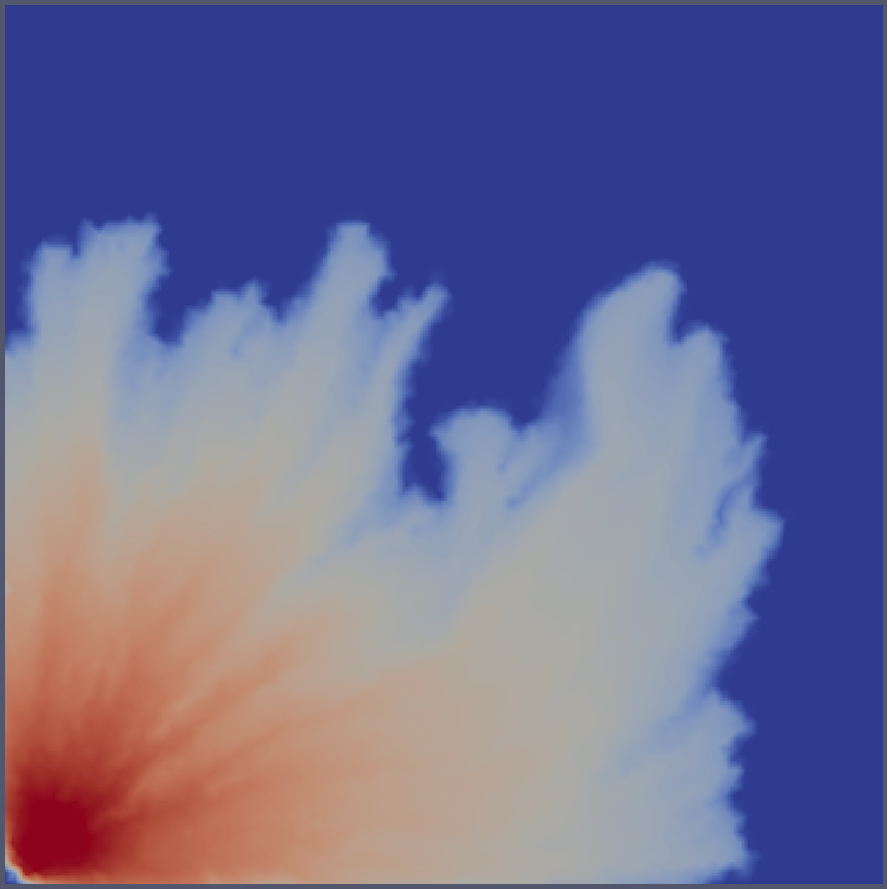
\includegraphics[width=.5\textwidth]{./Pics1/Saffman_heterogeneous/saffman_heter_fixed_3000.pdf}
            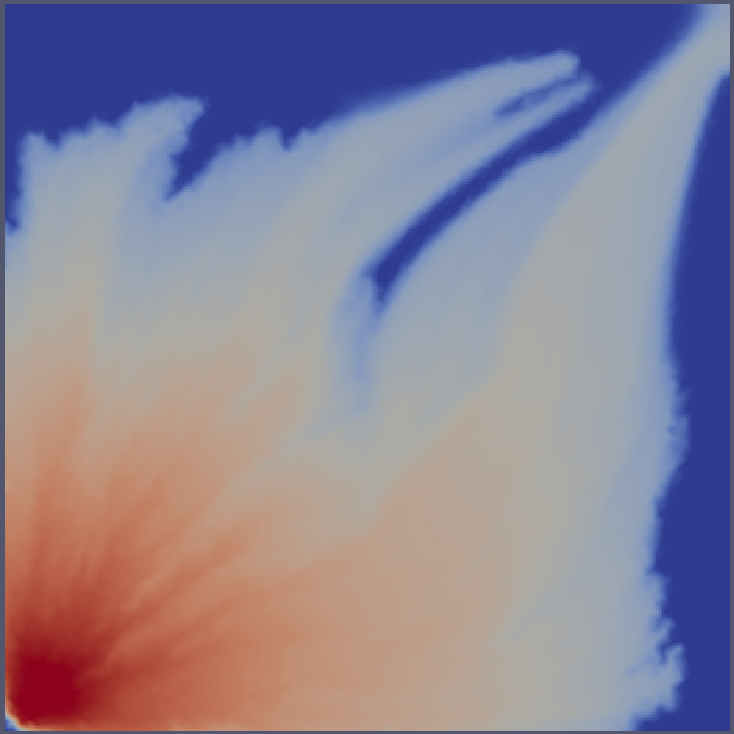
\includegraphics[width=.5\textwidth]{./Pics1/Saffman_heterogeneous/saffman_heter_fixed_6000.pdf}
            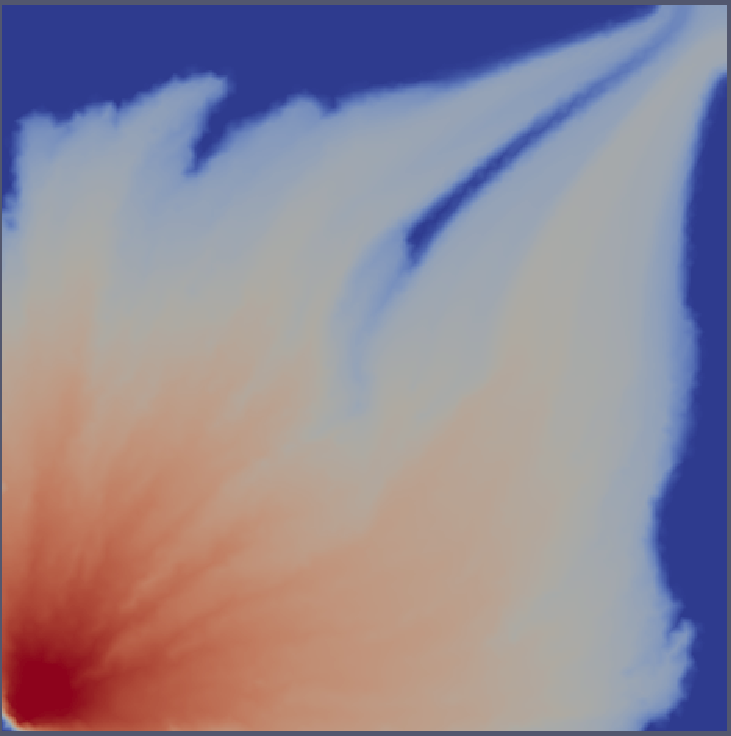
\includegraphics[width=.5\textwidth]{./Pics1/Saffman_heterogeneous/saffman_heter_fixed_24000.pdf} }
      \hbox{\hspace{2.5cm} (d) t=18s \hspace{5.cm} (e) t= \hspace{3.0cm} (f) t=24000 }}
\caption{Simulated flow in a modified Hele-Shaw cell with {\it VR}=10: (a) permeability distribution $\left(\text{10}^{-10}\le\mathbf{K}_{1}\le\text{5}\times\text{10}^{-10}\right.$, {\bf K}$_{2}$=10$^{-10}$, 10$^{-11}\le\mathbf{K}_{3}\le$ 5$\times$10$^{-10}$ and 10$^{-12}\le\mathbf{K}_{4}\le$ 5$\times$10$\left.^{-10}\text{ cm}^{2}\right)$; (b-f) snapshots of saturation profile during \red{XX} seconds of simulation. The domain contains \red{XX} \PN[1]{2} element-pairs.}
\label{fig:HeleShawHeter_VR10}
\end{figure}
\end{landscape}
\clearpage



%%%%
%%%%  FIGURE
%%%%
\begin{landscape}
\begin{figure}[ht] 
\vbox{
\hbox{\hspace{4.0cm}
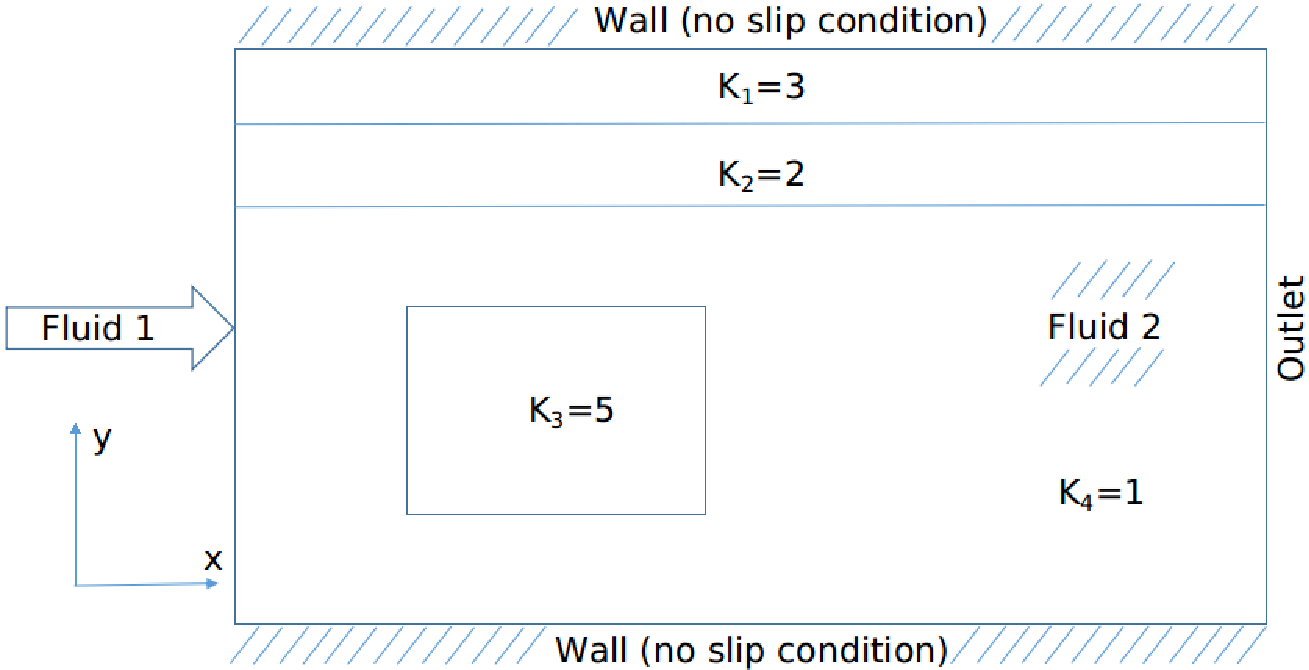
\includegraphics[width=.75\textwidth]{./Pics/map_of_boundaries.pdf} 
}
\vspace{0.0cm}
\hbox{\hspace{6.5cm} (a) map of permeabilties K   
}
\vspace{0.25cm}
\hbox{\hspace{4.0cm}
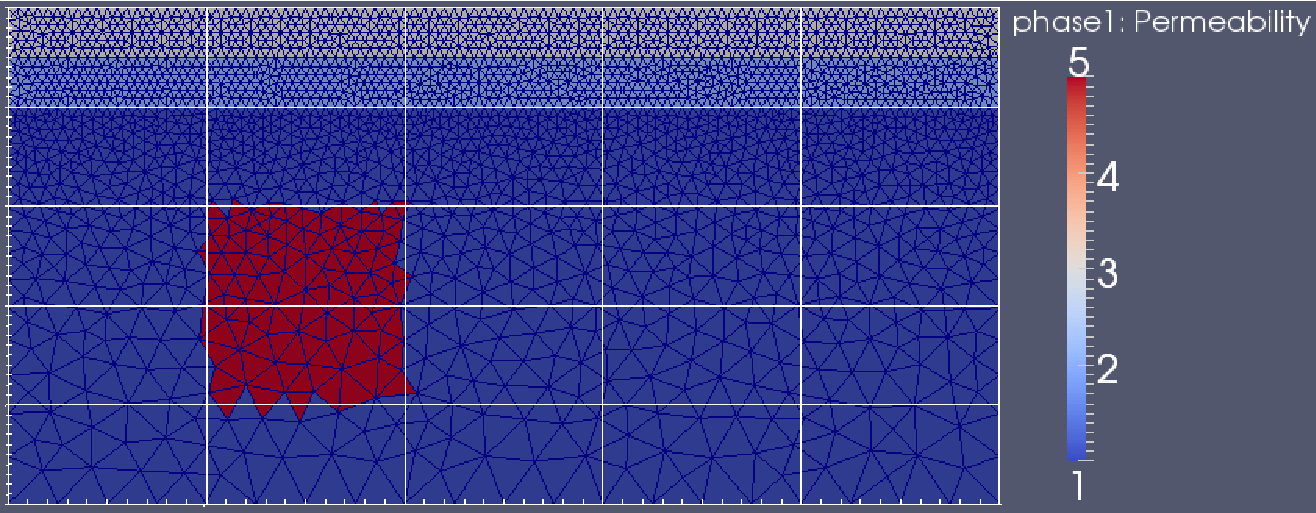
\includegraphics[width=.9\textwidth]{./Pics/map_of_boundaries_1.pdf}
}
\vspace{0.0cm}
\hbox{\hspace{9cm} (b)      
}
}     
\caption{Figure (a) describes the initial and boundary conditions as these are applied in this set of simulations. Below (b) there is a comparison between the unstructured and fixed mesh and the unstructured and adaptive mesh. During the implementation of fixed mesh initially there $4606$ elements while for the adaptive mesh there are $606$ while the majority of them is on the interface between between the two fluids. }
\label{fig:testcase_heter_domain}
\end{figure}
\end{landscape}
\clearpage



%%%%
%%%%  FIGURE
%%%%
\begin{landscape}
\begin{figure}[ht] 
\vbox{
\hbox{\hspace{3.5cm}
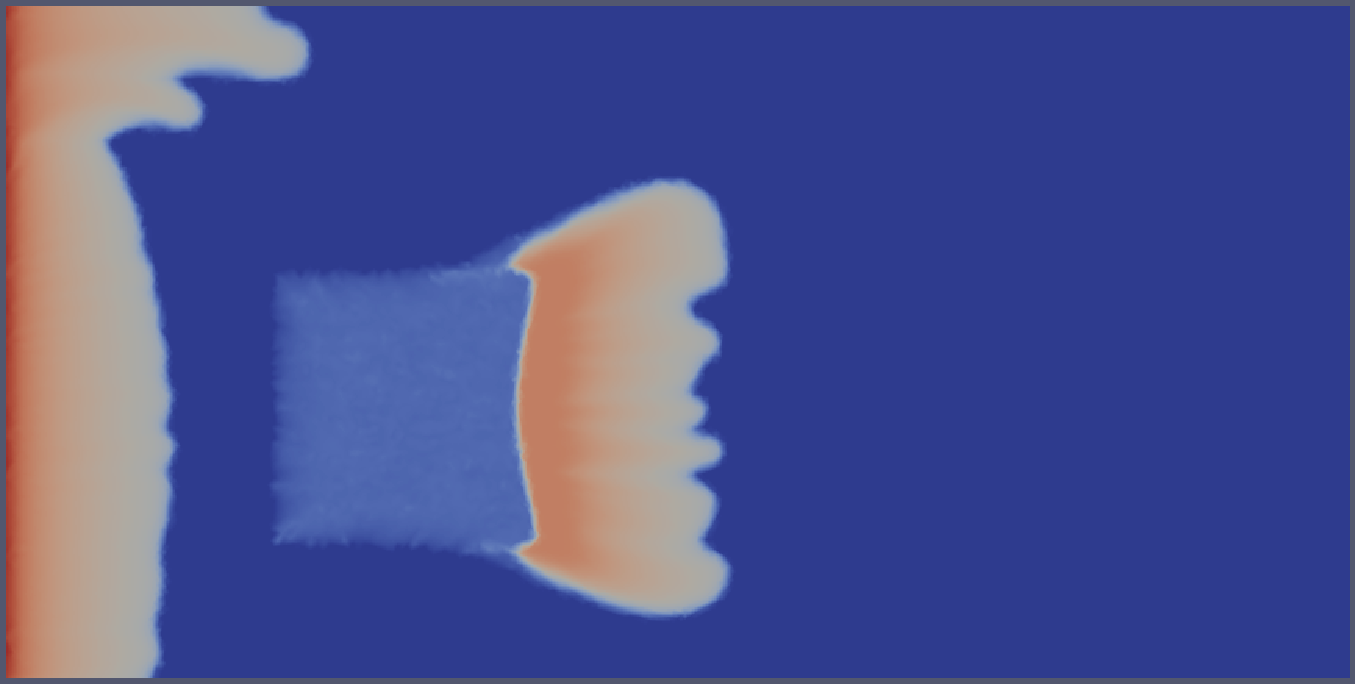
\includegraphics[width=.65\textwidth]{./Pics1/mr10_5regions_fixed/5regions_fixed_250.pdf} 
}
\vspace{0.0cm}
\hbox{\hspace{6.5cm} (a) flow at t=250 (fixed mesh)  
}
\vspace{0.25cm}
\hbox{\hspace{3.5cm}
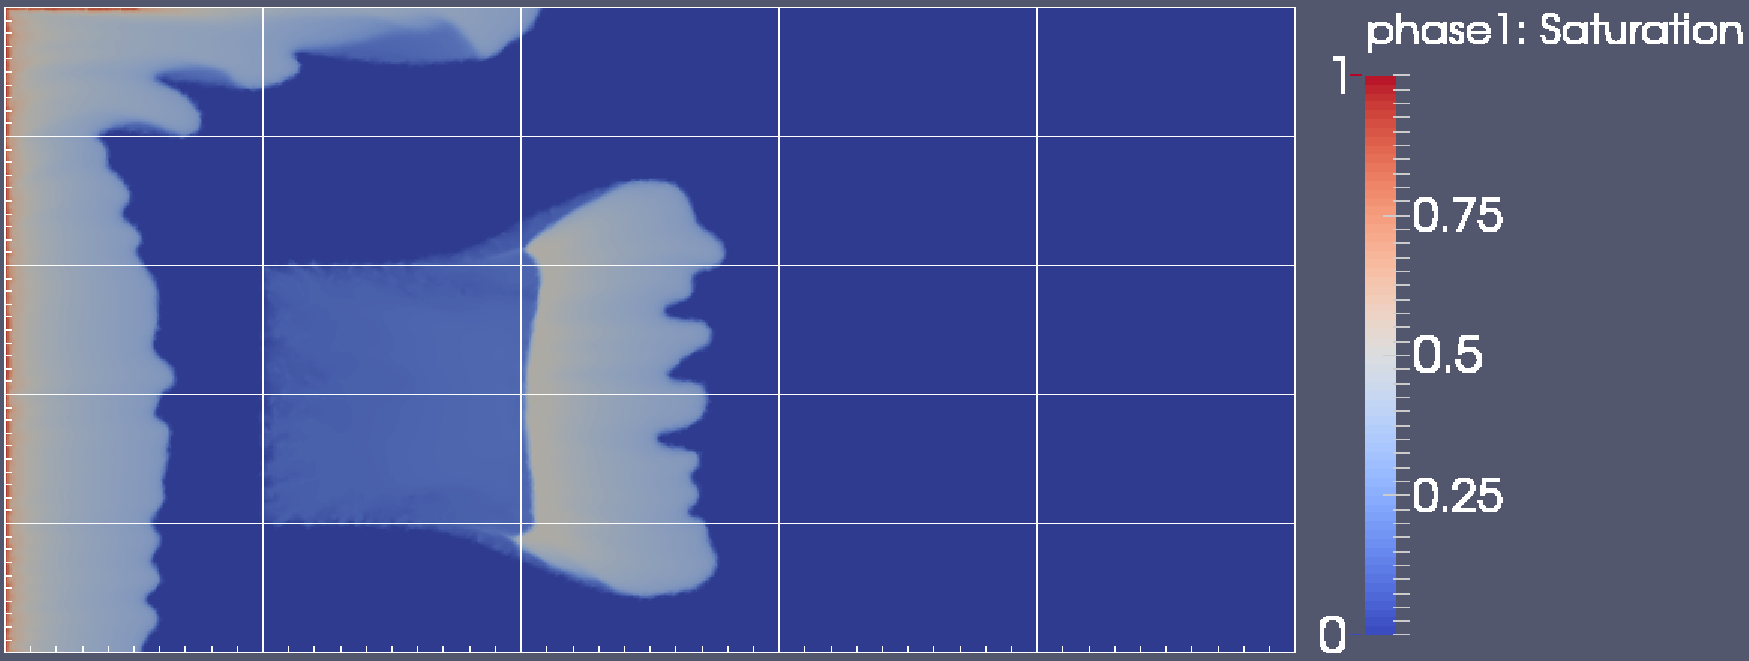
\includegraphics[width=.9\textwidth]{./Pics1/mr10_5regions_adapt/5regions_adapt_250_1.pdf}
}
\vspace{0.0cm}
\hbox{\hspace{6.5cm} (b) flow at t=250 (adaptive mesh)    
}
}     
\caption{For $t=0.125$s, $2$ test-cases under the VR=$10$ and under fixed (top) and adaptive(bottom) mesh are compared. There is a significant difference on the main front (left hand side of the domain) and the number of finger that appear.}
\label{fig:2testcase_a}
\end{figure}
\end{landscape}
\clearpage


%%%%
%%%%  FIGURE
%%%%
\begin{landscape}
\begin{figure}[ht] 
\vbox{
\hbox{\hspace{3.5cm}
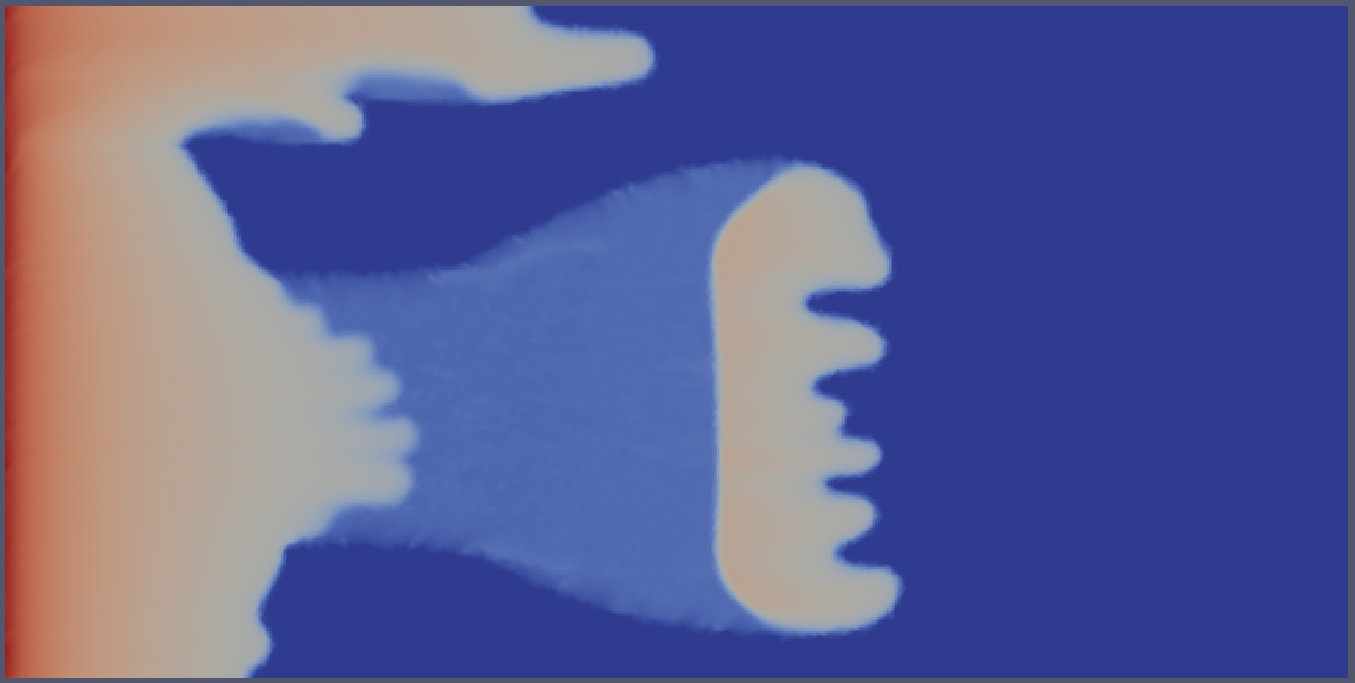
\includegraphics[width=.65\textwidth]{./Pics1/mr10_5regions_fixed/5regions_fixed_500.pdf} 
}
\vspace{0.0cm}
\hbox{\hspace{6.5cm} (a) flow at t=500 (fixed mesh)   
}
\vspace{0.25cm}
\hbox{\hspace{3.5cm}
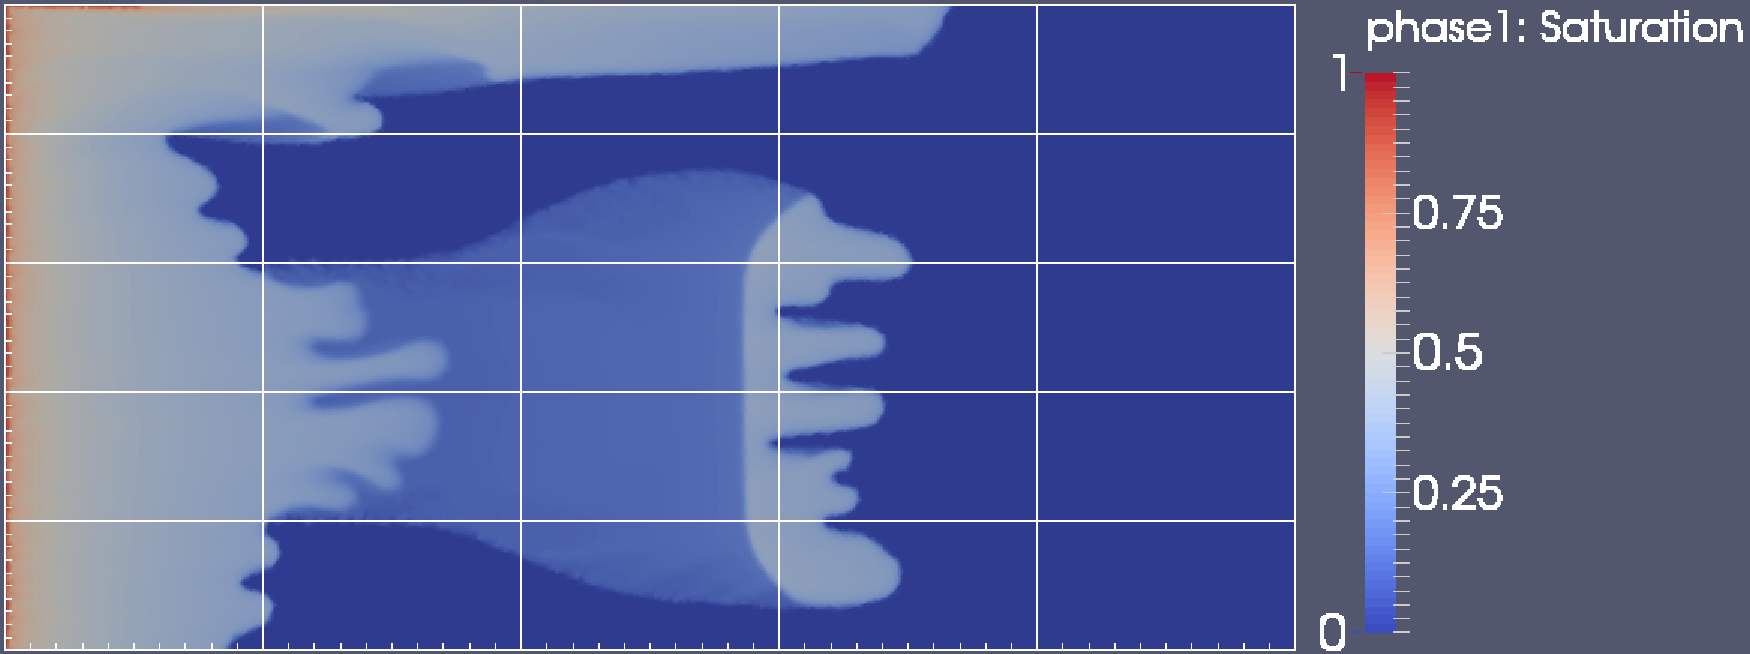
\includegraphics[width=.9\textwidth]{./Pics1/mr10_5regions_adapt/5regions_adapt_500_1.pdf}
}
\vspace{0.0cm}
\hbox{\hspace{6.5cm} (b) flow at t=500 (adaptive mesh)     
}
}     
\caption{At $t=0.25$s ($t=500$, timestemp) cross flow is taking place at the upper part of the formation. The fingers start to becoming more proufound as can been seen at the bottom.}
\label{fig:2testcase_b}
\end{figure}
\end{landscape}
\clearpage



%%%%
%%%%  FIGURE
%%%%
\begin{landscape}
\begin{figure}[ht] 
\vbox{
\hbox{\hspace{3.5cm}
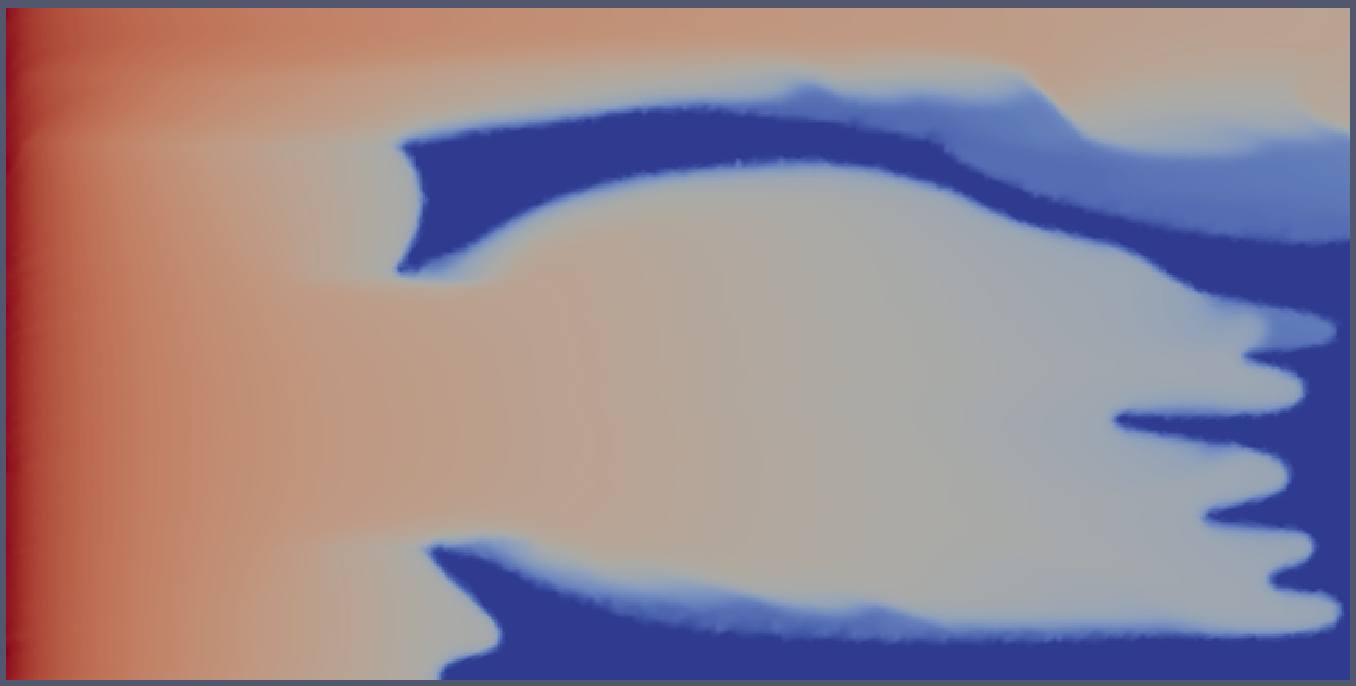
\includegraphics[width=.65\textwidth]{./Pics1/mr10_5regions_fixed/5regions_fixed_1500.pdf} 
}
\vspace{0.0cm}
\hbox{\hspace{6.5cm} (a) flow at t=1500 (fixed mesh)   
}
\vspace{0.25cm}
\hbox{\hspace{3.5cm}
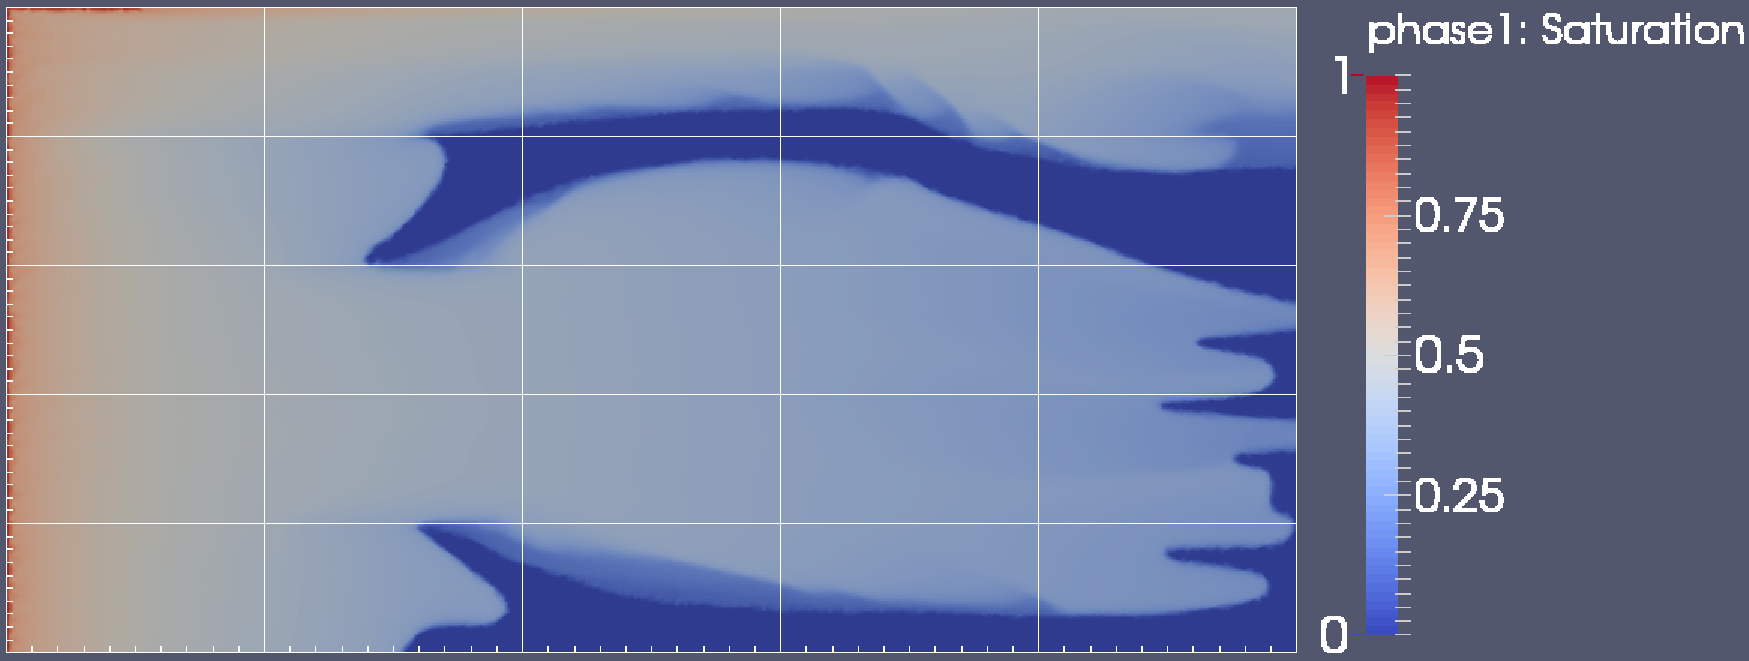
\includegraphics[width=.9\textwidth]{./Pics1/mr10_5regions_adapt/5regions_adapt_1500_1.pdf}
}
\vspace{0.0cm}
\hbox{\hspace{6.5cm} (b) flow at t=1500 (adaptive mesh)     
}
}     
\caption{At $t=0.75 sec$ ($t=1500$, timestemp) the initial cross flow is now fully developed and has travel all the way towards the outlet (right-hand side). and the finger below start forming a front that is also travelling towards the left-hand side.}
\label{fig:2testcase_c}
\end{figure}
\end{landscape}
\clearpage



%%%%
%%%%  FIGURE
%%%%
\begin{landscape}
\begin{figure}[ht] 
\vbox{
\hbox{\hspace{3.5cm}
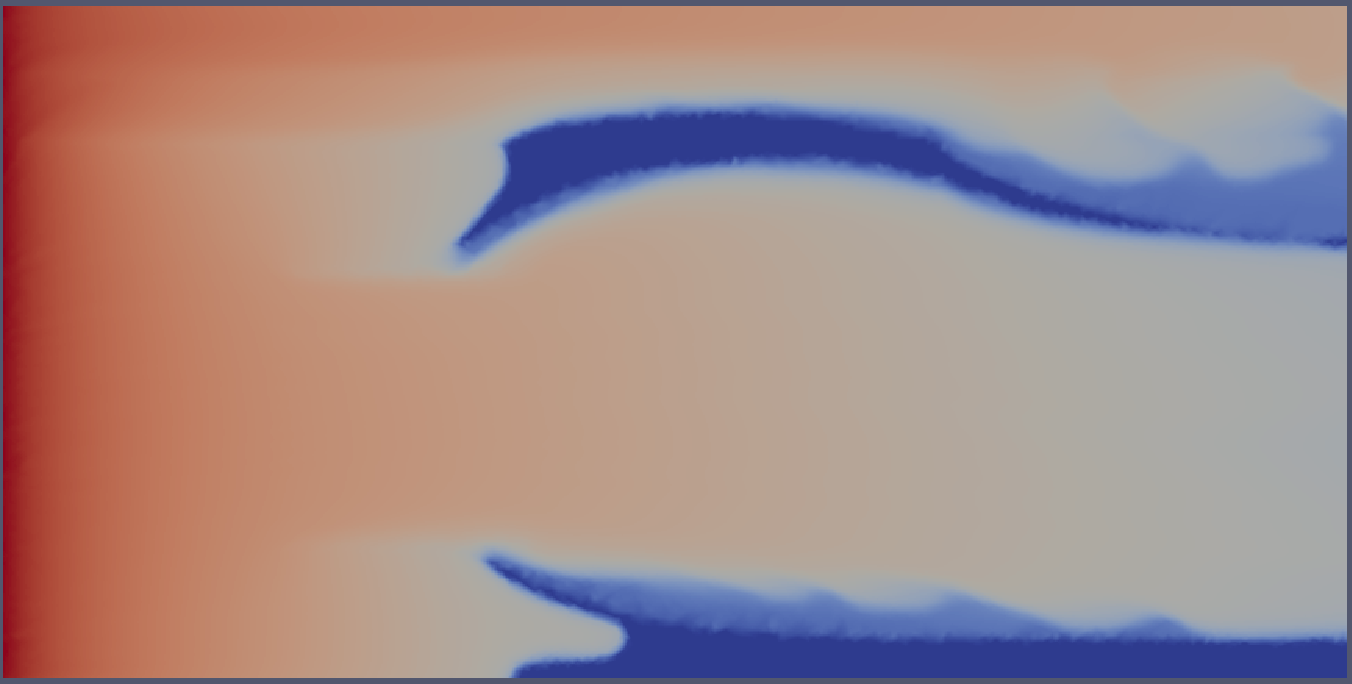
\includegraphics[width=.65\textwidth]{./Pics1/mr10_5regions_fixed/5regions_fixed_2000.pdf} 
}
\vspace{0.0cm}
\hbox{\hspace{6.5cm} (a) flow at t=end (fixed mesh)   
}
\vspace{0.25cm}
\hbox{\hspace{3.5cm}
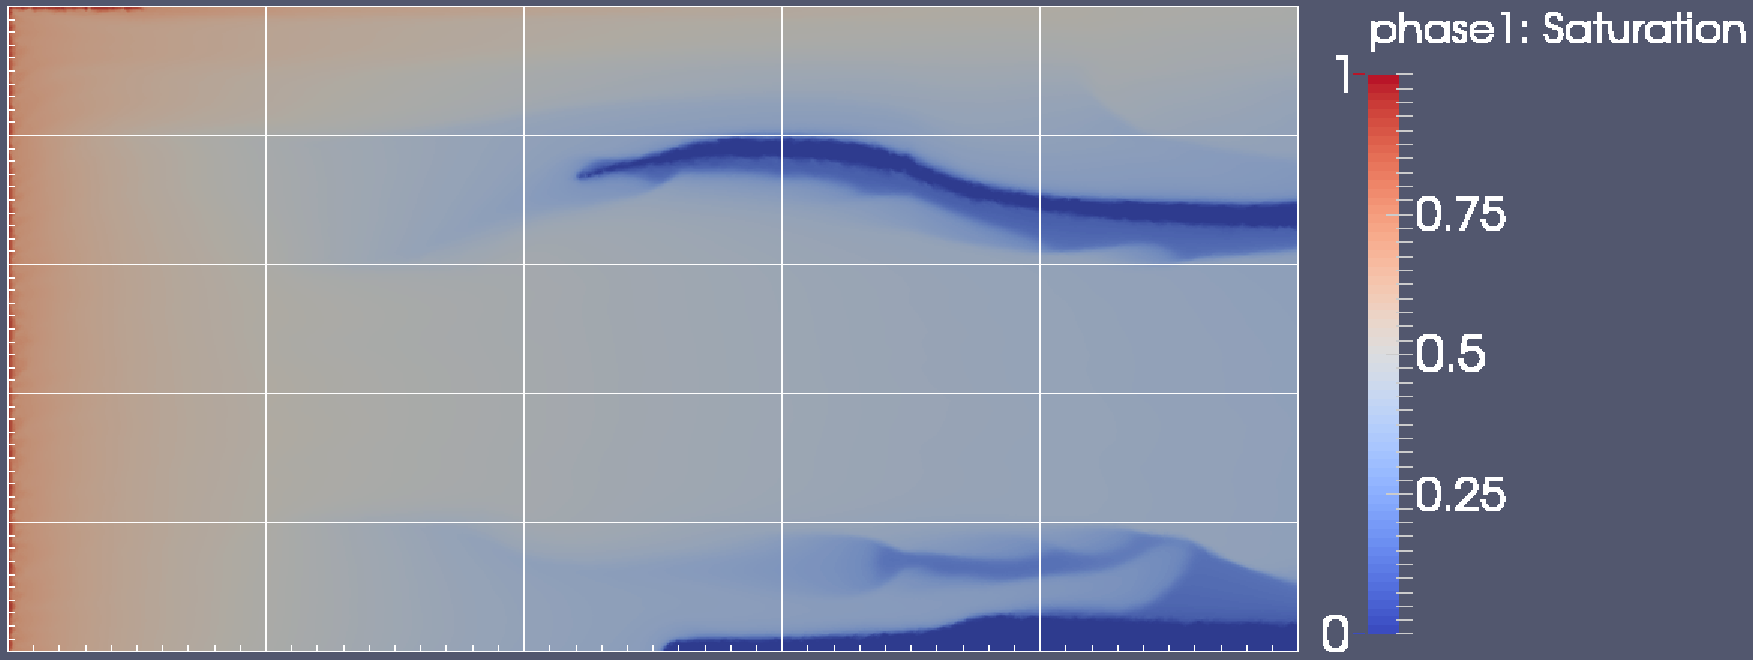
\includegraphics[width=.9\textwidth]{./Pics1/mr10_5regions_adapt/5regions_adapt_3000_1.pdf}
}
\vspace{0.0cm}
\hbox{\hspace{6.5cm} (b) flow at t=end (adaptive mesh)     
}
}     
\caption{Using the $P_{1}DGP_{2}$ element type for VR=$10$ under the same time steps, we compared the impact of fixed and adaptive mesh for the same timeframe. The end of simulation happens at $time=5 sec$ and for the timestemp $t=9999$ while the number of elements in both simulations was approximately $4700$. When adaptive mesh is introduce there is better repersentation of the fluid instabilities as these are developed on time.}
\label{fig:2testcase_d}
\end{figure}
\end{landscape}
\clearpage



%%%%
%%%%  FIGURE
%%%%
\begin{landscape}
\begin{figure}[ht] 
\vbox{
\hbox{\hspace{3.5cm}
\includegraphics[width=.9\textwidth]{./Pics1/mr10_5regions_fixed_dinlet/5regions_dinlet_fixed_100_1.pdf}
}
\vspace{0.0cm}
\hbox{\hspace{6.5cm} (a) double inlet - fixed mesh   
}
\hbox{\hspace{3.5cm}
  \includegraphics[width=.67\textwidth]{./Pics1/mr10_5regions_adapt_dinlet/5regions_dinlet_adapt_start.pdf}
}
\vspace{0.0cm}
\hbox{\hspace{6.5cm} (b) double inlet adaptive mesh   
}
}     
\caption{Comparing test-cases of fixed and adaptive mesh while a second region/inlet is introduced. For $t=0.101$s, using the $P_{1}DGP_{2}$ element type for MR=$10$ under the same time steps. For this simulation there are $13226$ elements for the fixed messh and $43716$ for the adaptive.}
\label{fig:3testcase_a}
\end{figure}
\end{landscape}
\clearpage

%%%%
%%%%  FIGURE
%%%%
\begin{figure}[ht] 
\vbox{
\hbox{\hspace{3.5cm}
\includegraphics[width=.5\textwidth]{./Pics1/mr10_5regions_adapt/5regions_adapt_vel_magn.pdf} 
}
\vspace{0.0cm}
\hbox{\hspace{5.0cm} (a) single inlet velocity magnitude   
}
\hbox{\hspace{3.5cm}
\includegraphics[width=.5\textwidth]{./Pics1/mr10_5regions_adapt_dinlet/5regions_dinlet_adapt_vel_magn.pdf}
}
\vspace{0.0cm}
\hbox{\hspace{5.0cm} (b) double inlet velocity magnitude   
}
}     
\caption{For the same time step, t=1000, these plots describe the velocity magnitudes of the phase $1$ (injected fluid) under the same boundary and initiall conditions. From top to bottom,these graphs describe the velocity magnitude %for fixed mesh is plotted(top), the velocity magnitude 
for adaptive mesh-single inlet (top) and the velocity magnitude for adaptive mesh with double inlet (bottom) as these are also presented in fig.\ref{fig:3testcase_a}. The main difference between the upper and lower plot %is not just the ability to capture in greater detail, the fluid instabilities as they happenduring the finger development and their velocity patterns. While there 
is the impact of the second injection interval as this can be seen from the slope and the rate that the velocity magnitude is changing.}
\label{fig:vel_magn}
\end{figure}

%%%%
%%%%  FIGURE
%%%%
\begin{landscape}
\begin{figure}[ht] 
\vbox{
\hbox{\hspace{3.5cm}
\includegraphics[width=.65\textwidth]{./Pics1/5reg_dinlet_fixed_500.pdf} 
}
\vspace{0.0cm}
\hbox{\hspace{6.5cm} (a) double inlet - fixed mesh   
}
\hbox{\hspace{3.5cm}
\includegraphics[width=.9\textwidth]{./Pics1/5reg_dinlet_adapt_500_1.pdf}
}
\vspace{0.0cm}
\hbox{\hspace{6.5cm} (b) double inlet adaptive mesh   
}
}     
\caption{For $t=5$s there is a comparison between fixed mesh(a) and adaptive mesh(b).}
\label{fig:3testcase_b}
\end{figure}
\end{landscape}
\clearpage

%%%%
%%%%  FIGURE
%%%%
\begin{landscape}
\begin{figure}[ht] 
\vbox{
\hbox{\hspace{3.5cm}
\includegraphics[width=.65\textwidth]{./Pics1/5reg_dinlet_fixed_1500.pdf} 
}
\vspace{0.0cm}
\hbox{\hspace{6.5cm} (a) double inlet - fixed mesh   
}
\hbox{\hspace{3.5cm}
\includegraphics[width=.9\textwidth]{./Pics1/5reg_dinlet_adapt_1500_1.pdf}
}
\vspace{0.0cm}
\hbox{\hspace{6.5cm} (b) double inlet adaptive mesh   
}
}     
\caption{For $t=7.5$s this is a comparison between fixed mesh(a) and adaptive mesh(b).}
\label{fig:3testcase_c}
\end{figure}
\end{landscape}
\clearpage

%%%%
%%%%  FIGURE
%%%%
\begin{landscape}
\begin{figure}[ht] 
\vbox{
\hbox{\hspace{3.5cm}
\includegraphics[width=.65\textwidth]{./Pics1/5reg_dinlet_fixed_end.pdf} 
}
\vspace{0.0cm}
\hbox{\hspace{6.5cm} (a) double inlet - fixed mesh   
}
\hbox{\hspace{3.5cm}
\includegraphics[width=.9\textwidth]{./Pics1/5reg_dinlet_adapt_end_1.pdf}
}
\vspace{0.0cm}
\hbox{\hspace{6.5cm} (b) double inlet adaptive mesh   
}
}     
\caption{This is a comparison between fixed mesh(a) and adaptive mesh(b) at the end of the simulation. For the fixed mesh at this point the maximum number of point is $13226$ while for the adaptive mesh is $7582$ and most of them are located where is needed in the domain.}
\label{fig:3testcase_d}
\end{figure}
\end{landscape}
\clearpage

%%%%
%%%%  FIGURE
%%%%
\begin{landscape}
\begin{figure}[ht] 
\vbox{
\hbox{\hspace{3.5cm}
\includegraphics[width=.8\textwidth]{./Pics1/mr100_fixed/mr100_fixed_500.pdf} 
}
\vspace{0.0cm}
\hbox{\hspace{4.0cm} (a) fixed and unstructured mesh for MR = 100 (start)   
}
\hbox{\hspace{3.5cm}
\includegraphics[width=.8\textwidth]{./Pics1/mr100_fixed/mr100_fixed_1500.pdf}
}
\vspace{0.0cm}
\hbox{\hspace{3.75cm} (b) fixed and unstructured mesh for MR = 100 (t = 1500)   
}
}     
\caption{For the case of VR=$100$ from top to bottom, the number of elements is $4680$ and fixed and unstructured mesh for the same time steps, t=$0.25$ or t=500(a), t=$0.75$ or t=1500(b). }
\label{fig:4testcase_a}
\end{figure}
\end{landscape}
\clearpage

%%%%
%%%%  FIGURE
%%%%
\begin{landscape}
\begin{figure}[ht] 
\vbox{
\hbox{\hspace{3.5cm}
\includegraphics[width=.8\textwidth]{./Pics1/mr100_fixed/mr100_fixed_3000.pdf} 
}
\vspace{0.0cm}
\hbox{\hspace{3.75cm} (c) fixed and unstructured mesh for MR = 100    
}
\hbox{\hspace{3.5cm}
\includegraphics[width=.8\textwidth]{./Pics1/mr100_fixed/mr100_fixed_end.pdf}
}
\vspace{0.0cm}
\hbox{\hspace{7.cm} (d) end of simulations     
}
}     
\caption{screenshot (c) is for t=$1.5$ sec or t=$3000$ and screenshot (d) is for t=$3.175$ sec, at the end of the simulations. }
\label{fig:4testcase_b}
\end{figure}
\end{landscape}
\clearpage



%\input{Manuscript_Figure1}

%%%%%%%%%%%%%%%%%%%%%%%%%%%%%%%%%%%%%%%%%%%%%%%%%%%%%%%%%%%%%%%%%%%%%%%%%%%%%%%%%%%%%%%%%%%%%%%%%%%%%%%%%%%%%%%%%%%%%%%%%%%%%%%%%%%%%%%%%%%%%%%%%%%%%%%%%%%%%%%%%%%%%%%%%%%%%%%%%%%%%%%%%%%%%%%%%%%%
\section{Results}\label{section:results}

%%%%%%%%%%%%
\subsection{Model Validation}

The set of test-cases that we are going to illustrate starts with an elementary case in an homogeneous domain. The aim of this test-case is to verify that the numerical model is actually working in different simulation/scenarios starting from the basic ones. One step before it is important to verify the existence of cross flow in the following domain as this is defined in fig. \ref{fig:simple_case}. Fluid $1$ is introduced on the  across the left hand side of the formation. Later different mobility ratios and different regions of various permeabilities will be introduced, but for now only few of these initial and boundary conditions will be applied. 

\begin{figure}[h]
\begin{center}
\includegraphics[width=0.75\textwidth]{./Pics/phase_vol_frac_uni_perm_1.pdf}
\caption{This is the case where the initially piston shape front is collapsing and starts forming fingers in an unstructured domain with uniform permeability (on average 3000 elements).}
\label{fig:simple_case}
\end{center}
\end{figure}

\noindent One more case to demonstrate the model validation against experiments is described in fig. \ref{fig:square}. A square shape formation consisted of $4$ square regions that each one has $2$ values of different permeabilities (K is represented by the blue and red shaded square areas). The aspect ratio of the domain is $1$ and is fully saturated with fluid $2$. At the upper and lower sides of the domain no-slip boundary condition is applied, that at a solid boundary, the fluid will have zero velocity relative to the boundary. The fluid velocity at all fluid–solid boundaries is equal to that of the solid boundary.. The left hand side of the domain is defined as the inlet for fluid $1$ with a velocity of $u=1$ while the right hand side is the outlet and pressure is set to $0$. Fluid $1$ across the left hand side of the formation is trying to displace the existing fluid $2$. What can been seen here is a cross flow case as the flow passes through different regions and develops. The front start to collapse at the first half of the lenght D (D:distance) of the domain ($x= \frac{1}{2} D)$.

\begin{figure}[h]
\begin{center}
\subfigure[Initial and boundary conditions]{\includegraphics[width=0.65\textwidth]{./Pics/2b2_P1DGP2.pdf}\label{a}}
\subfigure[Plots of velocity magnitude, pressure and phase volume fraction]{\includegraphics[width=0.6\textwidth]{./Pics/2b2_P1DGP2_plot.pdf}\label{b}}
\caption{This is the first test-case of a square region with four subregions of constant permeabilities K. The mesh is unstructured but fixed and on average there are 5000 elements. Fluid $1$ is introduced from the right hand side at a constant velocity of u = 1, while as the flow progress the velocity magnitude drops to zero close to the outlet. This is a cross flow example based on the experimental work of \citet{evans_1994}. The main finger desrcibes the cross flow and starts to dies out during the transition from one permeability zone to another and as it approaches closer to the right boundary.}
\label{fig:square}
\end{center}
\end{figure}

\noindent In this test-case above the two phase volume volume fractions have the same but opposite behaviour across the length of the formation. The velocity magnitute is builded up starting from the inlet all the way to the middle of the square. There is a sharp pressure drop which is also an indication that the fluid 2 cannot be pushed any further (see fig.\ref{fig:square}) while the phase volume fraction is constant. An slightly modified test-case (see fig.\ref{fig:testcase}) follows with the initial and boundary condition to remain the same, but in this set of simulations the geometrical aspect ration is $2$. The last set of simulations as this is described in fig.\ref{fig:1testcase} is and extension of the previous case and the aim of is to verify the behaviour of the flow for two different mobility ratios of $1$ and $10$ respectively.

\begin{figure}[h]
\begin{center}
\subfigure[map of permeabilties K]{\includegraphics[width=0.75\textwidth]{./Pics1/2b2_wi_fine/2b2_whole_in_fine_perm_1.pdf}\label{a}}
\subfigure[flow at t=250]{\includegraphics[width=0.75\textwidth]{./Pics1/2b2_wi_fine/2b2_whole_in_fine_250_2.pdf}\label{b}}
\subfigure[flow at t=3000]{\includegraphics[width=0.75\textwidth]{./Pics1/2b2_wi_fine/2b2_whole_in_fine_3000_1.pdf}\label{c}}
\caption{In this test-case fixed and unstructured mesh is used. The aspect ratio is 2 (a), which allows the flow to develop for longer. Simulation time step increases from (b) to (c) and from t=250(start) to t=3000(end).}
\label{fig:testcase}
\end{center}
\end{figure}

 The purpose of these cases was to verify that our model is working for cases that experimentally are proven. This will allow to proceed further and expand this technique into more complex formations. A more detailed description of the element type and the formation that will be used in the next set of test cases follows.

\begin{figure}[h]
\makebox[\textwidth]{%
\subfigure[MR1]{%
\includegraphics[width=0.49\textwidth]{./Pics1/mr1_fixed/mr1_fixed_100_2.pdf}%
}%
\hfill    
\subfigure[MR10]{%
\includegraphics[width=0.49\textwidth]{./Pics1/mr10_fixed/mr10_fixed_100_1.pdf}%
}}\\[0.5cm]% If you want some vertical space
\makebox[\textwidth]{%
\subfigure[MR1]{%
\includegraphics[width=0.49\textwidth]{./Pics1/mr1_fixed/mr1_fixed_middle_1.pdf}%
}%
\hfill    
\subfigure[MR10]{%
\includegraphics[width=0.49\textwidth]{./Pics1/mr10_fixed/mr10_fixed_middle_1.pdf}%
}}\\[0.5cm]% If you want some vertical space
\makebox[\textwidth]{%
\subfigure[MR1]{%
\includegraphics[width=0.49\textwidth]{./Pics1/mr1_fixed/mr1_fixed_end_2.pdf}%
}%
\hfill    
\subfigure[MR10]{%
\includegraphics[width=0.49\textwidth]{./Pics1/mr10_fixed/mr10_fixed_end_2.pdf}%
}}%
\caption{Comparing MR1 and MR10 cases using fixed mesh. Simulation time step increases from top to bottom and from (a) t=100(start) to (c) t=3000(end).}
\label{fig:1testcase}
\end{figure}


%%%%%%%%%%%%
\subsection{Hele-Shaw verification cases for homogeneous and heterogeneous domains under two different mobility ratios}

\medskip
At this point we have to mentioned one more set of simulations, based on the work of \citet{saffman_1986}. The Hele-shaw cell geometrical domain as this is defined by experimental studies and is presented in figures \ref{fig:1a_homoheleshaw_3}, \ref{fig:1b_homoheleshaw_3} and fig. \ref{fig:1c_homoheleshaw_3} is used. In all cases, simulations were performed in a squared geometry of $5x5$, where fluid $1$ is added into the domain at the bottom left-hand side corner with a velocity (magnitude) of 0.7071 (i.e., sqrt(2*0.25)). The sink (represented by 0 pressure BC) is allocated in the top right hand side corner of the domain. Newmann BC (i.e., no flux) was imposed to all borders of the domain except at the top righ hand side corner. The mobility ratios for these $3$ cases are $3$ and $10$ while for the latter homogeneous and heterogeneous domain is used.  

\begin{figure}
\centering
\subfigure[Hell-Shaw cell domain]{\includegraphics[width=0.5\textwidth]{./Pics1/Saffman_homogeneous_MR3/saffman_homo_fixed_1.pdf}}\\[2mm]%
\subfigure[flow at t=250]{\includegraphics[width=0.5\textwidth]{./Pics1/Saffman_homogeneous_MR3/saffman_homo_fixed_250.pdf}}%
\caption{This is a description of a Hele-Shaw experimental domain, showing the source and sink term as this is implied in this test-case followed by a screenshot of the flow at time, t=250(b). More screenshot follow that describe the progression of the flow in fig.\ref{fig:1b_homoheleshaw_3} and fig.\ref{fig:1c_homoheleshaw_3}}
\label{fig:1a_homoheleshaw_3}
\end{figure}

\begin{figure}
\centering
\subfigure[flow at t=1000]{\includegraphics[width=0.5\textwidth]{./Pics1/Saffman_homogeneous_MR3/saffman_homo_fixed_1000.pdf}}\\[2mm]%
\subfigure[flow at t=2500]{\includegraphics[width=0.5\textwidth]{./Pics1/Saffman_homogeneous_MR3/saffman_homo_fixed_2500.pdf}}%
\caption{As the flow progress, t=1000(a), a tip start to appears, at t=2500(b)}
\label{fig:1b_homoheleshaw_3}
\end{figure}

\begin{figure}
\centering
\subfigure[flow at t=3500]{\includegraphics[width=0.5\textwidth]{./Pics1/Saffman_homogeneous_MR3/saffman_homo_fixed_3500.pdf}}\\[2mm]%
\subfigure[flow at t=end]{\includegraphics[width=0.5\textwidth]{./Pics1/Saffman_homogeneous_MR3/saffman_homo_fixed_end_1.pdf}}%
\caption{This tip will become sharper at t=3500(a) as it approaches the area where sink term exist and finally at t=end(b) it will be absorbed.}
\label{fig:1c_homoheleshaw_3}
\end{figure}

%%%%%%%%%%%%%
\begin{figure}
\centering
\subfigure[Hell-Shaw cell domain]{\includegraphics[width=0.5\textwidth]{./Pics1/Saffman_homogeneous/saffman_homo_fixed_1.pdf}}\\[2mm]%
\subfigure[flow at t=250]{\includegraphics[width=0.5\textwidth]{./Pics1/Saffman_homogeneous/saffman_homo_fixed_250_1.pdf}}%
\caption{This is a description of a Hele-Shaw experimental domain, when MR=$10$ showing the source and sink term as this is implied in this test-case followed by a screenshot of the flow at time, t=250(b). Screenshot will follow that describe the progression of the flow in fig.\ref{fig:2b_homoheleshaw_10} and fig.\ref{fig:2c_homoheleshaw_10}}
\label{fig:2a_homoheleshaw_10}
\end{figure}

\begin{figure}
\centering
\subfigure[flow at t=1000]{\includegraphics[width=0.5\textwidth]{./Pics1/Saffman_homogeneous/saffman_homo_fixed_1000.pdf}}\\[2mm]%
\subfigure[flow at t=4000]{\includegraphics[width=0.5\textwidth]{./Pics1/Saffman_homogeneous/saffman_homo_fixed_4000.pdf}}%
\caption{As the flow progress at t=1000(a) the front still remains uniform. The first break down of the front is happening at t=4000(b) where $3$ tips start to come out of the main flow.}
\label{fig:2b_homoheleshaw_10}
\end{figure}

\begin{figure}
\centering
\subfigure[flow at t=6000]{\includegraphics[width=0.5\textwidth]{./Pics1/Saffman_homogeneous/saffman_homo_fixed_6000.pdf}}\\[2mm]%
\subfigure[flow at t=end]{\includegraphics[width=0.5\textwidth]{./Pics1/Saffman_homogeneous/saffman_homo_fixed_end_1.pdf}}%
\caption{Finger are now more obvious as the flow progress and the tip-splitting mechanism becomes stronger at t=6000(a) as it approaches the area where sink term exist and finally at t=end(b) it will be absorbed.}
\label{fig:2c_homoheleshaw_10}
\end{figure}

%%%%%%%%%%%%%
\begin{figure}
\centering
\subfigure[Hell-Shaw cell domain]{\includegraphics[width=0.5\textwidth]{./Pics1/Saffman_heterogeneous/saffman_heter_fixed_1.pdf}}\\[2mm]%
\subfigure[flow at t=250]{\includegraphics[width=0.5\textwidth]{./Pics1/Saffman_heterogeneous/saffman_heter_fixed_500.pdf}}%
\caption{This is a description of a heterogeneous Hele-Shaw experimental domain, when MR=$10$ showing the source and sink term as this is implied in this test-case followed by a screenshot of the flow at time, t=500(b). Screenshot will follow that describe the progression of the flow in fig.\ref{fig:3b_heteheleshaw_10} and fig.\ref{fig:3c_heteheleshaw_10}}
\label{fig:3a_heteheleshaw_10}
\end{figure}

\begin{figure}
\centering
\subfigure[flow at t=2000]{\includegraphics[width=0.5\textwidth]{./Pics1/Saffman_heterogeneous/saffman_heter_fixed_2000.pdf}}\\[2mm]%
\subfigure[flow at t=3000]{\includegraphics[width=0.5\textwidth]{./Pics1/Saffman_heterogeneous/saffman_heter_fixed_3000.pdf}}%
\caption{As the flow progress at t=2000(a) but now the front is completely unstable as it has already collapsed forming many finger formations. Finger formations are more aggressive as the simulations progress, t=3000(b) where many tips have already start to develop out of the main flow.}
\label{fig:3b_heteheleshaw_10}
\end{figure}

\begin{figure}
\centering
\subfigure[flow at t=6000]{\includegraphics[width=0.5\textwidth]{./Pics1/Saffman_heterogeneous/saffman_heter_fixed_6000.pdf}}\\[2mm]%
\subfigure[flow at t=24000]{\includegraphics[width=0.5\textwidth]{./Pics1/Saffman_heterogeneous/saffman_heter_fixed_24000.pdf}}%
\caption{At t=6000(a), one main finger have already reached the area where sink exists as they have develop much faster than the rest of the fingers. At t=24000(b) there are two main fingers that now have developed and drive the flow forwards.}
\label{fig:3c_heteheleshaw_10}
\end{figure}

%{./Pics/P1DG-P2_element_type} 
%{./Pics/4r_po_adapt_fine_125_mesh} 
%{./Pics/4r_po_adapt_fine_100_mesh}

%%%%%%%%%%%%%
\subsection{\blue{need to find a name for this heterogeneus region/set of test-cases for MR10 fixed vs. adaptive mesh}}

\medskip
\KCnote{ 4regions and 4 permeabilities}
\noindent Having already verified that model is working for the hele-shaw experimental test-cases, now a more complicated case will be introduced with regions of different geometrical domains and different permeabilities. There is a significant growth of fingers when comparing mobility ratios that differ an order of magnitude (Fig.\ref{fig:1testcase}) so the next step is a comparison under the same mobility ratio of $10$, using the fixed and the adaptive mesh test case. Figure \ref{fig:testcase_heter_domain} gives a description of the domain that will be used. Figures \ref{fig:2testcase_a}, \ref{fig:2testcase_b}, \ref{fig:2testcase_c}, \ref{fig:2testcase_d} will give a description of th esimulation for different time-steps as these are desrcibed. In this set the interfacial instability is becoming more profound. Based on these two case so far, an initial relation between the quantitative and qualitative outcome of our simulations can be derived. Fingers will develop faster in areas where permeabilities are higher. This can be seen from the overall sharp increase of velocity magnitude during the injection of the fluid $1$.    

\begin{figure}[h]
\begin{center}
\subfigure[map of permeabilties K]{\includegraphics[width=0.75\textwidth]{./Pics/map_of_boundaries.pdf}\label{a}}
\subfigure[permeabilities using an unstructured and fixed computational domain]{\includegraphics[width=0.75\textwidth]{./Pics/4r_po_adapt_fine_125_mesh.pdf}\label{b}}
\caption{(a) describes the initial and boundary conditions as these are applied in this set of simulations. Below (b) the unstructured and fixed mesh can been seen and there is a colored representation of permeabilities.}
\label{fig:testcase_heter_domain}
\end{center}
\end{figure}

\begin{figure}
\centering
\subfigure[flow at t=250 (fixed mesh)]{\includegraphics[width=0.75\textwidth]{./Pics1/mr10_5regions_fixed/5regions_fixed_250.pdf}}\\[2mm]%
\subfigure[flow at t=250 (adaptive mesh)]{\includegraphics[width=0.75\textwidth]{./Pics1/mr10_5regions_adapt/5regions_adapt_250.pdf}}%
\caption{Start to compare $2$ test-cases under MR=$10$ and under fixed (top) and adaptive(bottom) mesh for t=250. There is a significant difference on the main front (left hand side of the domain) and the number of finger that appear.}
\label{fig:2testcase_a}
\end{figure}

\begin{figure}
\centering
\subfigure[flow at t=500 (fixed mesh)]{\includegraphics[width=0.75\textwidth]{./Pics1/mr10_5regions_fixed/5regions_fixed_500.pdf}}\\[2mm]%
\subfigure[flow at t=500 (adaptive mesh)]{\includegraphics[width=0.75\textwidth]{./Pics1/mr10_5regions_adapt/5regions_adapt_500.pdf}}%
\caption{Cross flow is taking place at the upper part of the formation. The fingers start to becoming more proufound for for the (b) case below.}
\label{fig:2testcase_b}
\end{figure}

\begin{figure}
\centering
\subfigure[flow at t=1500 (fixed mesh)]{\includegraphics[width=0.75\textwidth]{./Pics1/mr10_5regions_fixed/5regions_fixed_1500.pdf}}\\[2mm]%
\subfigure[flow at t=1500 (adaptive mesh)]{\includegraphics[width=0.75\textwidth]{./Pics1/mr10_5regions_adapt/5regions_adapt_1500.pdf}}%
\caption{Cross flow at the upper part has almost travel all the way towards the outlet (left-hand side) and the finger below start forming a general trend/front that is also travelling towards the left-hand side.}
\label{fig:2testcase_c}
\end{figure}

\begin{figure}
\centering
\subfigure[flow at t= end (fixed mesh)]{\includegraphics[width=0.75\textwidth]{./Pics1/mr10_5regions_fixed/5regions_fixed_2000.pdf}}\\[2mm]%
\subfigure[flow at t= end (adaptive mesh)]{\includegraphics[width=0.75\textwidth]{./Pics1/mr10_5regions_adapt/5regions_adapt_3000.pdf}}%
\caption{Using the $P_{1}DGP_{2}$ element type for MR=$10$ under the same time steps, we compared the impact of fixed and adaptive mesh. When adaptive mesh is introduce there is better repersentation of the fluid instabilities as these are developed on time.}
\label{fig:2testcase_d}
\end{figure}

%%%%%%%%%%%%%
\subsection{\blue{need to find a name for this heterogeneus region/set of test-cases for MR10 adaptive double inlet}}

\medskip
\KCnote{velocity magnituted comparison under the adaptive vs. adaptive and refined mesh - NOT sure if we can include that}

%\begin{figure}
%\centering
%\subfigure[flow at t=1000  (adaptive coarse mesh)]{\includegraphics[width=0.75\textwidth]{./Pics1/mr10_4regions_python_only_adapt/4regions_python_only_coarse_vel_magn.pdf}}\\[2mm]%
%\subfigure[flow at t=1000  (adaptive and fine mesh)]{\includegraphics[width=0.75\textwidth]{./Pics1/mr10_4regions_python_only_adapt/4regions_python_only_adapt_vel_magn.pdf}}\\[2mm]%
%\subfigure[flow at t=1000  (adaptive and refined mesh)]{\includegraphics[width=0.75\textwidth]{./Pics1/mr10_4regions_python_only_adapt/4regions_python_only_adapt_refine_vel_mag.pdf}}%
%\caption{For the same time step, t=1000, these plots describe the velocity magnitudes of the phase $1$ (injected fluid) under the same boundary and initiall conditions. From top to bottom These graphs describe the velocity magnitude for single inlet with adaptive and fine mesh (a) and adaptive and refined mesh (b). The main difference between the (a) and (b) lies in the first part and how the velocity magnitude is builded up as a relation of phase $1$ volume fraction.}
%\label{fig:vel_magn1}
%\end{figure}

In fig.\ref{fig:3testcase_a} there is a set of simulations for when another region (inlet) of fluid $1$ ins introduced into the formation. This time fluid $1$ is injected from both the left hand side and the upper left corner of the domain, at a velocity u=$0.5$ while the set up of the problem remains the same, the mobility ratio is $10$, and the adaptive and ustructured mesh is implied. The top layer is saturated with phase $2$, while the rest of the domain has a saturation of $0.1$. The major difference is located in the velocity fields (see fig.\ref{fig:vel_magn2}) as the presence of this extra inlet increases the flow at the top layers. At this point is proper to mentioned the extreme case, see fig.{\ref{fig:4testcase}, when mobility ratio is even an order of magnitude higher, when MR=$100$. Even though a this case is unlikely to happen as the mobility ration of the existing fluids in the industry, it is a test-case that can illustrate the higher, faster and more profound development of instabilities. Also by focusing the grid resolution in the saturation front, \citet{christou2015}  demonstrated the explicit formation of fingers formed due to the instability in the pressure field and triggered by viscosity ratio. A comparison has also been made by using a low resolution element, the $P_{1}DG-P_{1}DG$. No fingers could be observed due to mesh coarseness (fingers were observed in finer uniform and adaptive meshes).

%%%%%%%%%%%%%
\begin{figure}
\centering
\subfigure[map of permeabilities]{\includegraphics[width=0.75\textwidth]{./Pics1/map_of_perm_1.pdf}}\\[2mm]%
\subfigure[flow at start]{\includegraphics[width=0.75\textwidth]{./Pics1/5reg_dinlet_adapt_100.pdf}}%
\caption{In fig.(a) there is the map of permeabilities as this will be implemented in this case while in fig.(b) there is an illustration of the adaptive mesh just in the beggining of the simulation.}
\label{fig:3testcase_a}
\end{figure}

\begin{figure}
\centering
\subfigure[dual inlet flow, fixed mesh, t=500]{\includegraphics[width=0.75\textwidth]{./Pics1/5reg_dinlet_fixed_500.pdf}}\\[2mm]%
\subfigure[dual inlet flow, adaptive mesh, t=500]{\includegraphics[width=0.75\textwidth]{./Pics1/5reg_dinlet_adapt_500.pdf}}%
\caption{In fig.(a)  fig.(b) .}
\label{fig:3testcase_b}
\end{figure}








%%%%%%%%%%%%%
\begin{comment}
%%%%%%%%%%%%%%%%%%%%%%%%%%%%%%%%%%%%%%%%%%%%%%%%%%%%%%%%%%%%%%%%%%%%%%%%%%%%%%%%%%%%%%%%%%%%%%%%%%%%%%%%%%%%%%%%%%%%%%%%%%%%%%%%%%%%%%%%%%%%%%%%%%%%%%%%%%%%%%%%%%%%%%%%%%%%%%%%%%%%%%%%%%%%%%%%%%%%
The first example is a simple comparison between two cases using fixed mesh and mobility ratios of $1$ and $10$ respectively. The aspect ratio of the $2D$ domain is 2 and it favors viscous fingering effects while temperature is not taken into account (assume isothermal environment) and gravity effects are negligible. Fluid $1$ is initially injected from the left hand side with velocity $u_{inj}=1$. The domain is fully saturated with fluid $2$. At the outlet (right hand side) boundary pressure levels are set to zero while no slip boundary conditions are implied at the upper and lower part of the formation. Fixed time step sizes of $1 \times 10^{-3}$ for both the fixed meshes and the CFL number for this set of simulations is $0.5$. The $P_{1}DGP_{2}$ element type with piecewise linear description of veleocity within each element and quadratic pressure representation as part of the OCVFEM method along with the discontinuous Galerkin method are implied and composing the mesh. Saturation is located at the pressure nodes. Five different regions of 5 distinct absolute permeabilities (K) are introduced (fig.\ref{fig:5regions_domain}). The red square region is saturated with a $50\%-50\%$ mixture of both phase $1$ and $2$. 

Two general behaviors for the interface may occur: (i) If a more viscous fluid displaces a less viscous one or a less viscous displaces a more viscous with a low average velocity, the interface is flat; (ii) if a less viscous fluid displaces a more viscous one with intermediate values of the average velocity, single or mutliple fingers will be observed.

This test-case serves as a base case for comparison between mobility (or viscocity) ratios that differ by an order of magnitude. Viscocity is a measure of resistance, therefore a frictional property. In these test-cases the $\sigma$ term as this is described above contains the individual parameters related with wettability and contact angle while the porous surface is a fluid $2$ wetted surface. For mobility ratios below $5$ the injection front will uniformly develop as time progress (piston shape front) and no fingers are expexted. Instabilities will start to occur and will be more obvious for mobility ratios higher than $5$. Between two layers or two regions with different permeabilities, but both saturated with fluid $2$, fingers will be triggered because of the permeability differences on the interface of these layers. In between the porous cappilary pressure difference with curve the interface and will lead to the formation of fingers. In macroscopic scale the interface between the two fluid will become unstable, an uneven or fingered profile will be controlled by capilary pressure -acting in the scale of the pores- and therefore due to the overall surface tension difference between the two immiscible fluids the front will collapse. This is of major practical importance in the petroleum industry, environmental waste remediation, and subsurface hydrology and it is key to understanding the movement of large volumes of injection fluids into subsurface reservoirs. The relationships between the capillarity of a geologic system, and the saturation and permeability of the fluids has a direct bearing on the migration speed and reservoir sweep of hydrocarbons affected the productivity of an oil field.

%%%%%%%%%%%%%%%%
\begin{figure}[h]
\makebox[\textwidth]{%
\subfigure[[MR10 fixed mesh start]{%
\includegraphics[width=0.49\textwidth]{./Pics1/mr10_5regions_fixed_dinlet/5regions_dinlet_fixed_100.pdf}%
}%
\hfill    
\subfigure[MR10 adapt mesh start]{%
\includegraphics[width=0.49\textwidth]{./Pics1/mr10_5regions_adapt_dinlet/5regions_dinlet_adapt_start.pdf}%
}}\\[0.5cm]% If you want some vertical space
\makebox[\textwidth]{%
\subfigure[MR10 fixed mesh t=1500]{%
\includegraphics[width=0.49\textwidth]{./Pics1/mr10_5regions_fixed_dinlet/5regions_dinlet_fixed_500.pdf}%
}%
\hfill    
\subfigure[MR10 adapt mesh t=1500]{%
\includegraphics[width=0.49\textwidth]{./Pics1/mr10_5regions_adapt_dinlet/5regions_dinlet_adapt_500.pdf}%
}}\\[0.5cm]% If you want some vertical space
\makebox[\textwidth]{%
\subfigure[MR10 fixed mesh t=7500]{%
\includegraphics[width=0.49\textwidth]{./Pics1/mr10_5regions_fixed_dinlet/5regions_dinlet_fixed_2000.pdf}%
}%
\hfill    
\subfigure[MR10 adapt mesh t=7500]{%
\includegraphics[width=0.49\textwidth]{./Pics1/mr10_5regions_adapt_dinlet/5regions_dinlet_adapt_2000.pdf}%
}}\\[0.5cm]% If you want some vertical space
\makebox[\textwidth]{%
\subfigure[MR10 fixed mesh end]{%
\includegraphics[width=0.49\textwidth]{./Pics1/mr10_5regions_fixed_dinlet/5regions_dinlet_fixed_end.pdf}%
}%
\hfill    
\subfigure[MR10 fixed adapt end]{%
\includegraphics[width=0.49\textwidth]{./Pics1/mr10_5regions_adapt_dinlet/5regions_dinlet_adapt_end.pdf}%
}}%
\caption{Comparing test-cases of fixed and adaptive mesh while we have a dual inlet, using the $P_{1}DGP_{2}$ element type for MR=$10$ under the same time steps, t=250(a,b), t=500(c,d), t=1500(e,f), t=3000(g,h). When adaptive mesh is introduce there is better repersentation of the fluid instabilities as these are developed on time.}
%\caption{Comparing the MR=$10$, between single and double injection of fluid $1$ under the adaptive and unstructured mesh for the same time steps, t=100(a,b), t=1500(c,d), t=7500(e,f), t=10000(g,h) }
\label{fig:3testcase}
\end{figure}


\begin{figure}
\begin{center}
%\includegraphics[width=0.5\textwidth]{./Pics1/mr10_5regions_fixed/5regions_vel_magn.png}\\[2mm]%
\includegraphics[width=0.49\textwidth]{./Pics1/mr10_5regions_adapt/5regions_adapt_vel_magn.pdf}\\[2mm]%
\includegraphics[width=0.49\textwidth]{./Pics1/mr10_5regions_adapt_dinlet/5regions_dinlet_adapt_vel_magn.pdf}%
\caption{For the same time step, t=1000, these plots describe the velocity magnitudes of the phase $1$ (injected fluid) under the same boundary and initiall conditions. From top to bottom,these graphs describe the velocity magnitude %for fixed mesh is plotted(top), the velocity magnitude 
for adaptive mesh-single inlet (top) and the velocity magnitude for adaptive mesh with double inlet (bottom) as these are also presented in fig.\ref{fig:3testcase}. The main difference between the upper and lower plot %is not just the ability to capture in greater detail, the fluid instabilities as they happen during the finger development and their velocity patterns. While there 
is the impact of the second injection interval as this can be seen from the slope and the rate that the velocity magnitude is changing.}
\label{fig:vel_magn2}
\end{center}
\end{figure}



%\begin{figure}
%\begin{center}
%\includegraphics[width=0.5\textwidth]{./Pics1/mr100_fixed/mr100_fixed_500.pdf}\\[2mm]%
%\includegraphics[width=0.5\textwidth]{./Pics1/mr100_fixed/mr100_fixed_1500.pdf}\\[2mm]%
%\includegraphics[width=0.5\textwidth]{./Pics1/mr100_fixed/mr100_fixed_3000.pdf}\\[2mm]%
%\includegraphics[width=0.5\textwidth]{./Pics1/mr100_fixed/mr100_fixed_end.pdf}%
%\caption{from top to bottom, these are screenshots taken from the test-case of MR=$100$ using fixed and unstructured mesh for the same time steps, t=500(a), t=1500(b), t=3000(c), t=end(d)}
%\label{fig:4testcase}
%\end{center}
%\end{figure}

\begin{comment}
\begin{figure}[h] 
\begin{center}
\subfigure[MR1]{%
\label{fig:}
\includegraphics[width=0.6\textwidth]{./Pics/MR1.pdf}
}%
\subfigure[Recovery for MR1]{%
\label{fig:}
\includegraphics[width=0.52\textwidth]{./Pics/Recovery_MR1_1.png}
}\\
\subfigure[MR10]{%
\label{fig:}
\includegraphics[width=0.6\textwidth]{./Pics/MR10.pdf}
}%
\subfigure[Recovery for MR10]{%
\label{fig:}
\includegraphics[width=0.52\textwidth]{./Pics/Recovery_MR10_10.pdf}
}\\
\subfigure[MR100]{%
\label{fig:}
\includegraphics[width=0.6\textwidth]{./Pics/MR100_100_start.pdf}
}%
\subfigure[Recovery for MR100]{%
\label{fig:}
\includegraphics[width=0.52\textwidth]{./Pics/Recovery_MR100_100.pdf}
}\\ 
\end{center}
\caption{Comparison of different MR's and their recovery rates. The comparison among the MR = $1$,MR = $10$ and MR = $100$ has been done using the boundary conditions and set upt as this has already been describe in the beginning of the section \ref{section:results}. }
\label{fig:recoveryrates}
\end{figure}
\end{comment}


The macroscopic sweep efficiency is principally affected by the heterogeneity in the reservoir which controls the spatial distribution of porosity and permeability. The permeability depends on the number, size and connectivity of the pores. This set of parameters is described by the $\sigma$ in the global mass balance equation (eq.\ref{global_mass_balance}). Including higher permeability zones also know as higher permeability channels or layers in the set up of the model, allows our test-cases to give a good approximation of the so called "thief zones", something that is common in heterogeneous geological formations. 
As can been seen so far in all the test-case illustrated, main differences can be found on the way the shape of fingering is developed. Adaptive meshes tend to display fingering easier because of the enhcanced and stronger resolution in the interface. Inside the high permeability square region there is an acceleration of the flow with the maximum value of it at the interface as this starts to develops at the back of this region and onwards. At this point attention should be given to the recovery rates as they can be illustrated from fig.{\ref{fig:recoveryrates}}. The breaking point, also known as the point the two curves meet where beyond that water production will occur, is shifted towards the right as MR is increased.

Even though the commercial simulators provide the user with option of an unstructured type of mesh still they are not able to dynamically adapt the mesh as the simulation develops and they increase the computational cost as the saturation front changes slowly. In this paper the use and benefits of dynamic mesh adaptivity to capture the viscous fingering in reservoir flows was introduced byt the use of OCVFEM and families of elements. Both the evolution of visualisation techniques through the extensive use of parallel computing as well as the advances in modelling and simulation of porous media flows may help to address the importance of this phenomenon which can be found in both upstream and downstream operations. Even thought this model is promising there is still work to be done since it is not yet a complete product. Further work is required to develop the surface-based modelling algorithms.


\section{Conclusions}

In conclusion the method that has been described in this paper as well as the simulations performed have a number of distinct advantages: 
\begin{enumerate}
\item[1.] The geological model can be designed from the beginning without any previous reference or geometrical limitations due to both the flexibility of method and to the fact that the geological characteristic and parameters can be easily introduced.
%\item[2.] Computational cost can be reduced because the complex geometries and surfaces are less expensive to generate and manage using fewer grid cells.
%\item[3.] The basis of the below argument is the flexibility and variance of the unstructured grid in time and space.
%\item[4.] Production simulations run directly on the geological model without the need to upscale.\\

\item[2.] The displacing fluid tends to flow easier towards the zones with higher values of permeability, as these can been seen from evolution of fingers in the upper layers of the domain. The higher the mobility ratio the easier it is for the uniform front of the injected fluid to break into fingers that eventually will decrease the recovery of hydrocarbon content.
\item[3.] The increased viscosity ratio increases the computational cost and requires the use of smaller time-step sizes. At the same time the basis of the argument above is the flexibility and variance of the unstructured grid in time and space. The domain used in these test-cases the development of the flow follow the linear tip-splitting finger behaviour.
\item[4.] Properties such as porosity and saturation can be readily up-scaled using statistical methods, can be included in the element boundaries,  while production simulations run directly on the geological model without the need to upscale.
\end{enumerate}


\begin{comment}
\begin{landscape}
\begin{figure}[ht!]
\begin{center}
\subfigure[MR100, at the beginning of the simulations]{%
\label{fig:1st}
\includegraphics[width=0.75\textwidth]{./Pics/4r_po_adapt_fine_100}
}%
\subfigure[MR100, at the middle of the simulation]{%
\label{fig:2nd}
\includegraphics[width=0.75\textwidth]{./Pics/4r_po_adapt_fine_125_phase1_vol_fraction_mesh}
}\\
\subfigure[MR100, Phase 1 Volume fraction]{%
\label{fig:3rd}
\includegraphics[width=0.75\textwidth]{./Pics/4r_po_adapt_fine_125_phase1_vol_frac}
}%
\subfigure[MR100, Phase 2 Volume fraction]{%
\label{fig:4th}
\includegraphics[width=0.75\textwidth]{./Pics/4r_po_adapt_fine_125_phase2_vol_fraction}
}\\
\caption{Comparison of different MR's and their recovery rates}
\label{fig:5}
\end{center}
\end{figure}
\end{landscape}
\end{comment}






\section{Achknowledgements}
Mr William Rad\"unz would like to acknowledge the support from the Brazilian Research Council (CNPq) under the \textit{Science without Borders scholarship programme}. Mr Konstantinos Christou would like to acknowledge the support of the University of Aberdeen - College of Physical Science as well as the Aberdeen Formation Evaluation Society (\textit{AFES}). Last but not least credit should be given to both Dr Jefferson Gomes \& Dr Marcus Campell Bannerman, both lecturers at the University of Aberdeen, at the School of Engineering.

\clearpage
\listoffigures

\clearpage 
%% References with bibTeX database:
\bibliographystyle{elsarticle-harv}
\bibliography{references}

\end{document}
%% End of tex file.

%%  LocalWords:  checkboard
